\section{Oscillation analysis}
\begin{figure}[h]
    \centering
    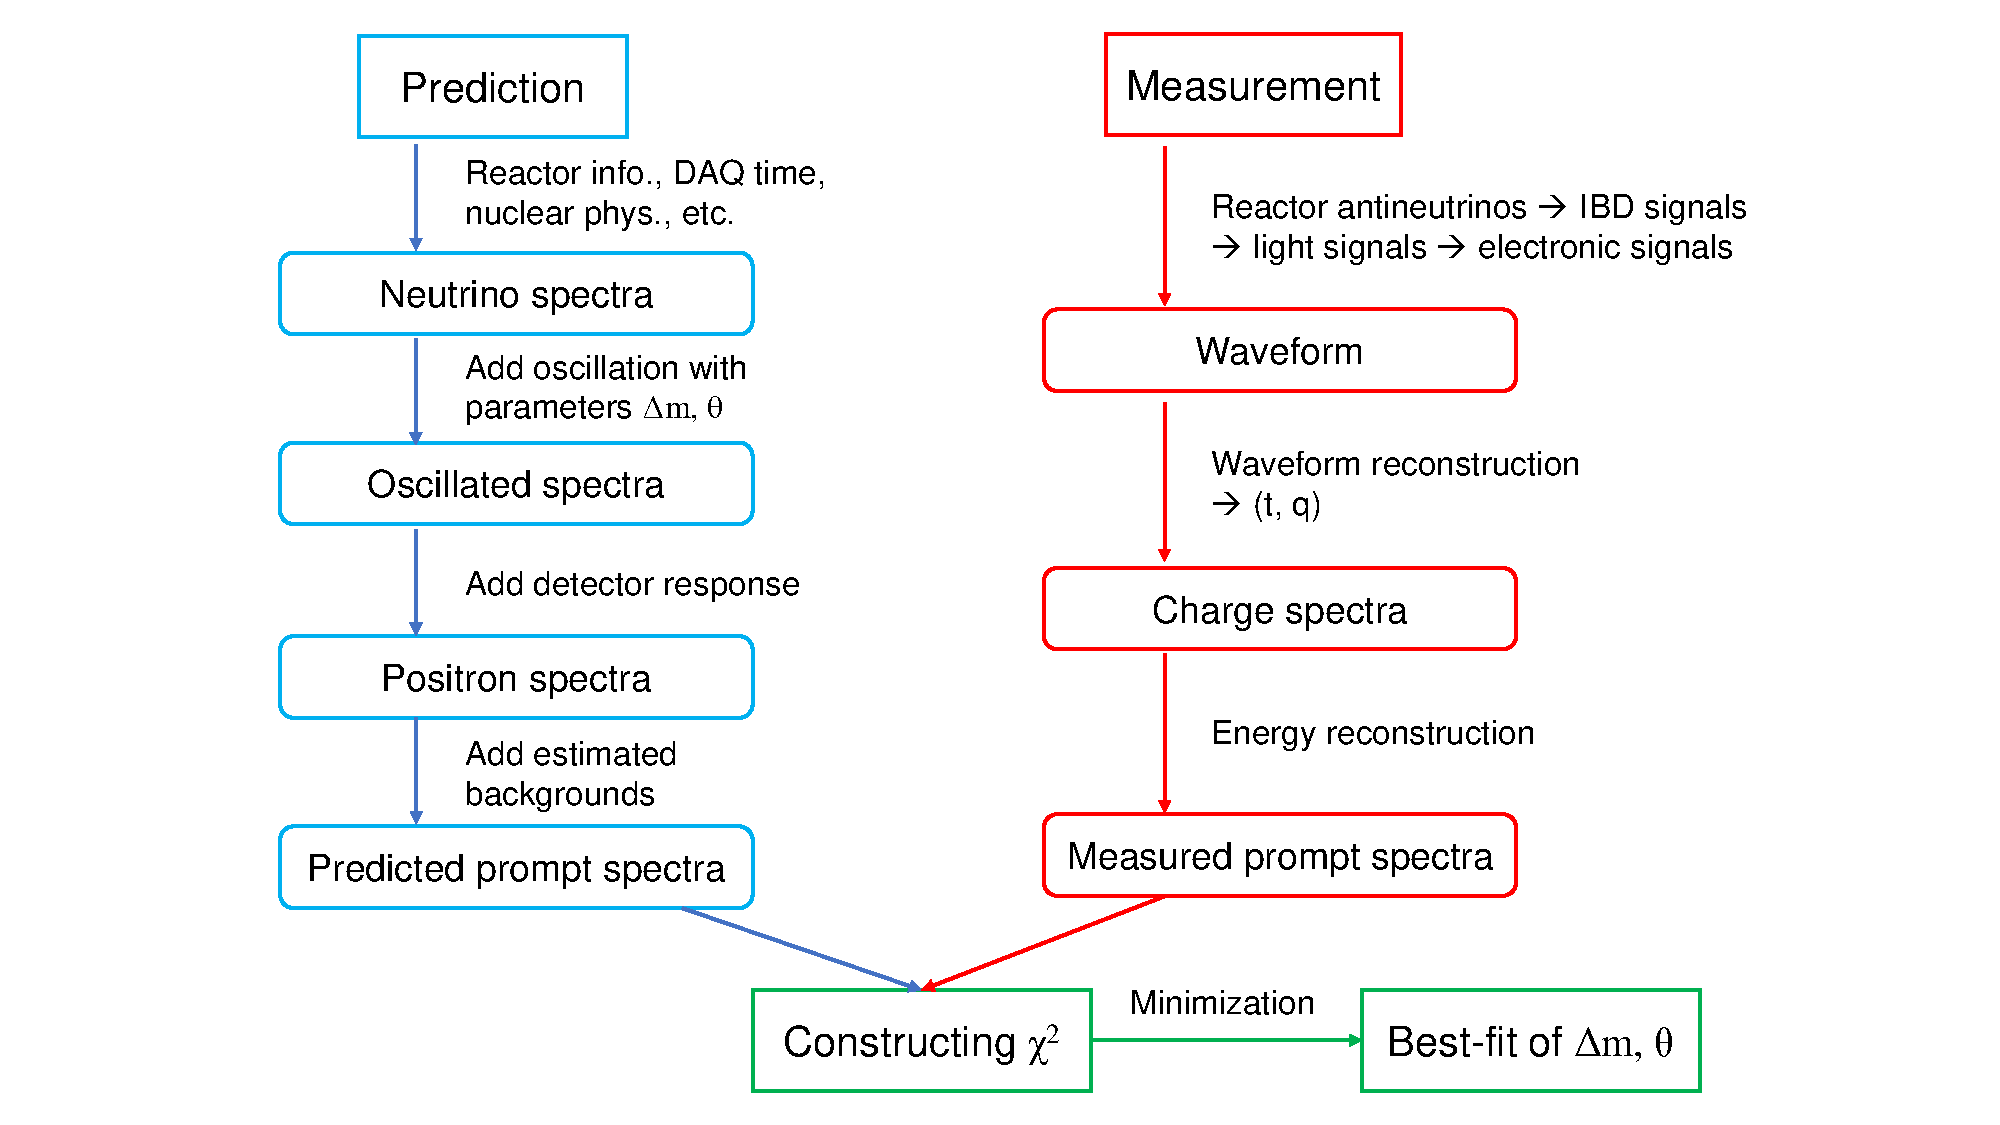
\includegraphics[width=16cm]{5_oscillation/oscAnaDiagram.pdf}
    \caption{Schematic diagram of the oscillation analysis.}
    \label{fig:oscAnaDiagram}
\end{figure}



\subsection{Statistical Analysis Framework}

This subsection defines the core statistical framework for extracting oscillation parameters
($\sin^2\theta_{12}$, $\Delta m^2_{21}$, $\Delta m^2_{31}$) from JUNO data.

\subsubsection{The statistical method}

We predict the binned reconstructed-energy spectrum $\boldsymbol{T}(\theta,\alpha)$ from
oscillation parameters $\theta$ and nuisance parameters $\alpha$ (detector, backgrounds, reactor),
where $\theta=(\sin^2\theta_{12},\Delta m^2_{21},\Delta m^2_{31},\sin^2\theta_{13})$.

With observed JUNO spectrum $\boldsymbol{M}$, We employ the least-squares method and construct a binned $\chi^2$ with pull terms to account for the impact of systematic uncertainties 
% \begin{equation}
%   \chi^2_{\mathrm{CNP}}(\theta,\nu) = \sum_i \frac{(n_i-\mu_i)^2}{\sigma_i^2}, \quad
%   \sigma_i^2 = \tfrac{1}{3}\,n_i + \tfrac{2}{3}\,\mu_i \label{eq:cnp}
% \end{equation}
\begin{equation}
    \begin{split}
        \chi^2_{\rm JUNO} \equiv &\sum_i^{Nbins}{\left(\frac{\left(M_i-T_i^{\rm IBD}\left(\alpha_C,\alpha_D,\alpha_l,\alpha_\eta,\dotsb\right)-\sum_B^{\rm Bkg}{\left(T_i^{B}(\alpha_B)\right)}\right)^2}{V_{ii}^{\rm stat}+\sum_B^{\rm Bkg}{\left(T_i^{B}(\alpha_B)\cdot \sigma_{\rm shp}^B\right)^2}})\right)}\\
        &+\left(\frac{\alpha_C}{\sigma_C}\right)^2+\sum_p^{\rm Plants}{\left(\frac{\alpha_{\rm Pow}^p}{\sigma_{\rm Pow}^p}\right)^2}+\sum_p^{\rm Plants}{\left(\frac{\alpha_{\rm SNF}^p}{\sigma_{\rm SNF}^p}\right)^2}+\sum_p^{\rm Plants}{\left(\frac{\alpha_{\rm NonEq}^p}{\sigma_{\rm NonEq}^p}\right)^2}+\frac{\boldsymbol{\alpha}_{\mathrm{FF}}^{\!\top}\,\boldsymbol{\rho}_{\mathrm{FF}}^{-1}\,\boldsymbol{\alpha}_{\mathrm{FF}}}{\sigma_{\mathrm{FF}}^{2}}\\
        &+\left(\frac{\alpha_D}{\sigma_D}\right)^2+\sum_{l=1}^{4}{\left(\frac{\alpha_l}{\sigma_l}\right)^2}+\left(\frac{\alpha_{\rm EScale}}{\sigma_{\rm EScale}}\right)^2+\sum_{\eta=a,b,c}\left(\frac{\alpha_{\eta}}{\sigma_{\eta}}\right)^2+\sum_{f=1}^{4}\left(\frac{\alpha_{\rm FE}^{f}}{\sigma_{\rm FE}^{f}}\right)^2\\
        &+\sum_B^{\rm Bkg}{\left(\frac{\alpha_B}{\sigma_B}\right)^2}+\left(\frac{\alpha_{\rm Th/U}}{\sigma_{\rm Th/U}}\right)^2+\sum_{k=1}^{5}{\left(\frac{\alpha^k_{\rm AtmShp}}{\sigma^k_{\rm AtmShp}}\right)^2}+\left(\frac{\alpha_{\rho ME}}{\sigma_{\rho ME}}\right)^2,
    \end{split}
    \label{eq:chisq:JUNO}
\end{equation}
where $M_i$ is measured total event number in i-the energy bin, which is the summation of signal and background. And $T_i^{\rm IBD}$ is the predicted IBD signal event number, which depends on the oscillation parameters of interest and will be described in Sec.~\ref{subsubsec:obs-spectrum}. $T_i^{B}$ is the estimated background event number of B-th kind of background, and the estimation procedure is listed in Sec.~\ref{sec:background}. The meaning of the indices in the chi-square formula are listed below:
\begin{itemize}
    \item i, refers to i-th energy bin;
    \item C, refers to reactor-related correlated uncertainty;
    \item D, refers to the detection efficiency uncertainty;
    \item B, refers to B-th background;
    \item l, refers to l-th liquid scintillator nonlinearity pull curve;
    \item EScale, refers to the absolute energy scale;
    \item $\eta$ (a,b,c) refers to energy resolution parameters;
    \item p, refers to p-th nuclear power plant;
    \item Pow, refers to thermal power;
    \item shp, refers to the spectrum shape uncertainties;
    \item $\rho_{ME}$, refers the matter density;
    \item NonEq, refers to the non-equilibrium;
    \item SNF, refers to the spent nuclear fuel;
    \item $\rm Th/U$, refers to the ratio of isotope Th to U for geo-neutrino;
    \item AtmShp, refers to the atmospheric-$\nu$ shape uncertainty;
    \item f, refers to 4 isotopes $^{235}U$, $^{238}U$, $^{239}Pu$, $^{241}Pu$;
    \item FF, refers to fission fractions for 4 isotopes;
    \item FE, refers to fission energy for 4 isotopes.
\end{itemize}
The $V_{ii}^{\rm stat}$ denotes statistical variance combines Neyman ($\sigma^2 \approx M$) and Pearson ($\sigma^2 \approx T$) statistics
\begin{equation}
    V_{ii}^{\rm stat}  \equiv 3\cdot\left(\frac{1}{M_i}+\frac{2}{T_i^{\rm IBD}+\sum_B^{\rm Bkg}T_i^{B}}\right)^{-1}\label{eq:Chisq:CNP},
\end{equation}
which exhibit biases in opposite directions. Their weighted combination eliminates first-order bias relative to the Poisson likelihood, improving parameter estimates while avoiding zero-bin failures.

The Daya Bay spectrum data are analyzed using a $\chi^2$ statistic constructed with the full covariance matrix:
% \begin{equation}
%   \chi^2_{\text{Pearson, DYB}} = \sum_k \frac{(n_k^{\text{DYB}}-\mu_k^{\text{DYB}})^2}{n_k^{\text{DYB}}} \label{eq:pearson}
% \end{equation}
\begin{equation}
    \chi^2_{\text{DYB}} = (\boldsymbol{M}^{\rm DYB} - \boldsymbol{T}^{\rm DYB})^T\mathbf{Cov}^{-1}(\boldsymbol{M}^{\rm DYB} - \boldsymbol{T}^{\rm DYB})\label{eq:Chisq:DYB},
\end{equation}
where $\boldsymbol{M}^{\rm DYB}$ is measured prompt energy spectrum from Ref.~\cite{DYB:Flux2025}, normalized to the spectrum per fission, after removing the effects of oscillation, spent nuclear fuel correction, and non-equilibrium correction. And $\boldsymbol{T}^{\rm DYB}$ is the predicted spectrum obtained using the detector response matrix from Ref.~\cite{DYB:Flux2025}, incorporating IBD cross section, liquid scintillator non-linearity, energy resolution, and inner acrylic vessel effect (IAV). Ref.~\cite{DYB:Flux2025} also provided the full covariance matrix $\mathbf{Cov}$ including statistical uncertainty and systematic uncertainties from detection, backgrounds, and reactors.

% External constraints enter as Gaussian pulls, with nuisance parameters $\alpha_j$ re-centered at zero:
% \begin{equation}
%   \chi^2_{\text{pull}} = \sum_j \left(\frac{\alpha_j}{\sigma_j}\right)^2 \label{eq:pull}
% \end{equation}

In addition to the pull terms for systematic uncertainties, external constraints on $\rm{sin}^2\theta_{13}$ and $\Delta m^2_{31}$ from the Daya Bay measurement~\cite{an2023precision} are also included in Sec.\ref{subsec:analysis:result}. The \textbf{total objective} to be minimized is therefore

\begin{equation}
\chi^2_{\text{Total}}
= \chi^2_{\text{JUNO}} + \chi^2_{\text{DYB}}
+ \left( \frac{\sin^2\theta_{13} - \sin^2\theta_{13}^{\rm DYB}}{\sigma(\sin^2\theta_{13}^{\rm DYB})} \right)^2
+ \left( \frac{\Delta m_{31}^2 - \Delta m_{31}^{2,\,\rm DYB}}{\sigma(\Delta m_{31}^{2,\,\rm DYB})} \right)^2 ,
\label{eq:Chisq:Total}
\end{equation}

\subsubsection{The observed spectrum prediction}
\label{subsubsec:obs-spectrum}
With the prompt energy distribution, we calculate the expected event number $T_{i}^{IBD}$ for i-th energy bin with Eq.~\eqref{eq:DetectorResponse:further}, which is needed for calculating the chi-square defined in Eq.~\eqref{eq:chisq:JUNO}.

\begin{equation}
    T_i^{IBD} \equiv (1+\alpha_C+\alpha_D)\cdot\int_{E^i_{\rm{rec}}}^{E^{i+1}_{\rm{rec}}}dE_{\rm{rec}}\int_{1.8}^{13} dE_{\bar{\nu}_e}\cdot S_0(E_{\bar{\nu}})\cdot R(E_{\bar{\nu}_e}, E_{\rm{rec}}),
    \label{eq:DetectorResponse:further}
\end{equation}
where $E_i$ and $E_{i+1}$ are the lower and upper edges of i-th energy bin, respectively. Both $\alpha_C$ and $\alpha_D$ are the nuisance parameters that float the overall normalization of the spectrum, corresponding to reactor-related correlated uncertainty and detection efficiency uncertainty, respectively. In the following, we sequentially describe the components of the expected antineutrino energy spectrum $S_0(E_{\bar{\nu}})$ arriving at JUNO, as well as the detector response function $R(E_{\bar{\nu}_e}, E_{\rm{rec}})$. 

The IBD signal detected at JUNO originates from ten reactor cores, whose effective thermal power, baselines, and effective fission fractions are summarized in Table~\ref{tab:ReactorInfo}. The effective thermal power and effective fission fractions are obtained by averaging the weekly reactor power and isotope-dependent fission numbers over the data-taking period. The IBD rate without selection efficiency for each core is also listed based on oscillation parameters from PDG 2024.

\begin{table}[ht]
    \centering
    \begin{tabular}{c|c|c|c|c|c|c|c}\hline
        Core    &   Power (GW)   &   Baseline (km)   &   $ff_{235U}$ &   $ff_{238U}$ & $ff_{239Pu}$ & $ff_{241Pu}$ & IBD rate ($\rm day^{-1}$)    \\ \hline
        TS-C1    & 4.09 & 52.77 & 0.670 & 0.076 & 0.223 & 0.031 & 8.53\\ 
        TS-C2    & 4.15 & 52.64 & 0.464 & 0.078 & 0.373 & 0.085 & 8.06\\ 
        YJ-C1    & 1.91 & 52.74 & 0.553 & 0.075 & 0.304 & 0.068 & 3.81\\ 
        YJ-C2    & 2.74 & 52.82 & 0.592 & 0.075 & 0.288 & 0.045 & 5.53\\ 
        YJ-C3    & 2.86 & 52.41 & 0.497 & 0.076 & 0.354 & 0.073 & 5.70\\ 
        YJ-C4    & 1.55 & 52.49 & 0.720 & 0.073 & 0.175 & 0.032 & 3.35\\ 
        YJ-C5    & 2.47 & 52.11 & 0.583 & 0.075 & 0.295 & 0.047 & 5.16\\ 
        YJ-C6    & 2.87 & 52.19 & 0.510 & 0.076 & 0.345 & 0.069 & 5.79\\ 
        DYB      & 15.90 & 215  & 0.549 & 0.076 & 0.315 & 0.060 & 3.37\\ 
        FCG      & 9.28 & 411   & 0.580 & 0.070 & 0.300 & 0.050 & 0.55\\ \hline
        All      & —     & —     & —     & —     & —     & —     & 49.84\\ \hline
    \end{tabular}
    \caption{Summary of unblind effective thermal power, baseline, effective fission fraction distribution of Yangjiang (YJ) and Taishan (TS) reactor complexes, as well as remote Daya Bay (DYB) reactor and Fangchenggang (FCG) reactor. }
    \label{tab:ReactorInfo}%
\end{table}%
The neutrino energy spectrum, $S_0(E_{\bar{\nu}_e})$ at JUNO in data-taking period, given by Eq.~\eqref{equ_generic}, is calculated with reactor antineutrino flux $\phi_r(E_{\nu})$ multiplied by electron antineutrino survival probability in Eq.~\eqref{eq:P_nue2nue}, with corresponding thermal power and baseline of the reactors.
\begin{equation}\label{equ_generic}
    S_0(E_{\nu},T_{\rm live})  = T_{\rm live} \cdot \sum_r \frac{P_{ee}(E_{\nu},L_{r})}{ 4\pi L^2_{r}}\phi_r(E_{\nu}),
\end{equation}
where $E_{\nu}$ is the $\bar\nu_e$ energy, $r$ is the reactor index, $L_{r}$ is the distance from detector to reactor $r$, $T_{\rm live}$ is the total DAQ live time, and $P_{ee}(E_{\nu},L_{r})$ is the $\bar{\nu}_e$ survival probability expressed as
\begin{equation}\label{eq:P_nue2nue}
    \begin{aligned}
        P_{\bar{\nu}_e\to\bar{\nu}_e}=1 & -\sin^22\theta_{13}(\cos^2\theta_{12}\sin^2\Delta_{31}+\sin^2\theta_{12}\sin^2\Delta_{32}) \\
                                        & -\cos^4\theta_{13}\sin^22\theta_{12}\sin^2\Delta_{21},
    \end{aligned}
\end{equation}
where $\Delta_{ji}=\Delta m_{ji}^2L/(4E)=(m_j^2-m_i^2)L/(4E)$, in which L is the baseline and E is antineutrino energy. The correction from matter effect~\cite{Khan:2019doq} on the survival probability is also included. The $\phi_r(E_{\nu})$ in Eq.\eqref{equ_generic} is the average antineutrino energy spectrum emitted per second from reactor $r$. 
\begin{equation}\label{equ_prediction}
    \phi_r(E_{\nu}) = \frac{W_r}{\sum_i f_{ir} \cdot e_i}\sum_i f_{ir} \cdot S_i(E_{\nu}),
\end{equation}
where $W_r(t)$ is the thermal power of reactor $r$, $e_i$ is the mean energy released per fission for isotope $i$, $f_{ir}(t)$ is the fission fraction. $S_i(E_{\nu})$ is the $\bar\nu_e$ energy spectrum per fission for i-th isotope, which is calculated by exponential interpolating the listed values from Huber in Ref.~\cite{Huber:2011wv} ($^{235}$U, $^{239}$Pu, and $^{241}$Pu) and Mueller in Ref.~\cite{Mueller:2011nm} ($^{238}$U). The values of fission fraction and fission energy used are listed in Table~\ref{tab:ReactorInfo}.
In the combined analysis using the JUNO and DYB near-detector measured spectra, the calculation of $\phi_r(E_{\nu})$ is modified accordingly. The detailed procedure for this modification, including the method for combining JUNO and DYB data, is described in Sec.~\ref{subsec:FluxInComb}.

The beta decay rate of some long-lived fission fragments will not reach equilibrium with their production rate. The non-equilibrium fission fragments will then accumulate in the reactor core, and their beta decay will contribute $\sim$0.6\% additional antineutrinos\cite{Mueller:2011nm}.

The burned nuclear fuel removed to a cooling pool near the reactor core is stored as spent nuclear fuel (SNF), the long-lived isotopes in which will also contribute $\sim$0.2\% additional antineutrinos in our analysis. Thus, the antineutrino energy spectrum $\phi_r(E_{\nu})$ is modified to cover the contributions of SNF and non-equilibrium (NonEq) effect as shown in Eq.~\eqref{eq:phi:SNF-NonEq}.
\begin{equation}
    \phi^\prime_r(E_{\nu})=\phi_r(E_{\nu})+\phi_r^{\rm HM}(E_{\nu}) \cdot f_{\rm NonEq}^r(E_{\nu})\cdot \left(1+\alpha_{\rm NonEq}^r\right)+\phi_{\rm SNF}^{r,\rm Abs}(E_{\nu})\cdot\left(1+\alpha_{\rm SNF}^r\right),
    \label{eq:phi:SNF-NonEq}
\end{equation}
where $f_{\rm NonEq}^r$ is the relative contribution of the NonEq effect to the antineutrion energy spectrum $\phi_r^{\rm HM}(E_{\nu})$ predicted by the Huber-Mueller model for reactor $r$, evaluated using the corresponding fuel history. The term $\phi_{\rm SNF}^{r,\rm Abs}(E_{\nu})$ gives the absolute SNF contribution per second derived from core simulation for reactor $r$. In particular, reactors YJ-C1 and YJ-C4 include an additional shutdown SNF component due to their recent shutdown operations.

For the part of detector response, we assume the energy leakage is negligibly small. Therefore, the deposited energy of positron $E_{\rm dep}$ in the liquid scintillator can be expressed in Eq.~\eqref{eq:E_dep}.

\begin{equation}
    % E_{\rm dep}=E_{e^+}+0.511\ {\rm{MeV}}.
    E_{\rm dep}=T_{e^+}+2\times0.511\ {\rm{MeV}},
    \label{eq:E_dep}
\end{equation}
where $T_{e^+}$ is the kinetic energy of positron. The positron energy $E_{e^+}=T_{e^+}+0.511~\rm{MeV}$ is function of the scattering angle $\cos\theta$ and antineutrino energy $E_{\bar{\nu}}$ in the IBD interaction. There are two widely used formulae of IBD cross-section. One is evaluated by Vogel and Beacom~\cite{Vogel:1999zy}, the other is calculated by Strumia and Vissani~\cite{Strumia:2003zx}. In this analysis, we adopt the Vogel–Beacom cross section for the prediction. Besides expressing the cross section in terms of the scattering angle, $\frac{d\sigma}{d\cos\theta}(E_{\bar{\nu}},\cos\theta)$, it can also be formulated as a function of the deposited energy through a variable substitution, $\frac{d\sigma}{dE_{e^+}}(E_{\bar{\nu}},E_{e^+})$~\cite{Vogel:1999zy}.
So the exact formula of the detector response function $R(E_{\bar{\nu}_e}, E_{\rm{rec}})$ in Eq.~\eqref{eq:DetectorResponse:further} can be expressed as Eq.~\eqref{eq:DetectorResponse:Full} shows.
\begin{equation}
    R(E_{\bar{\nu}_e}, E_{\rm{rec}}) \equiv \int_{0.8}^{12} dE_{\rm dep} \cdot \frac{d\sigma}{dE_{e^+}}(E_{\bar{\nu}},E_{e^+})
    \cdot N_p \cdot \epsilon \cdot
    \frac{1}{\sigma_{E_{\rm vis}}\sqrt{2\pi}}\cdot
    \exp{\left(-\frac{1}{2}\left(\frac{E_{\rm{rec}}-E_{\rm vis}\left(E_{\rm dep}\right)}{\sigma_{E_{\rm vis}}}\right)^2\right)},
    \label{eq:DetectorResponse:Full}
\end{equation}
where the prompt energy $E_{\rm{rec}}$ refers to the observed (smeared) visible energy of prompt signal, $N_p$ is the number of target proton number $(1.442\pm0.014)\times10^{33}$, and $\epsilon$ is the total IBD selection efficiency listed in Tabel~\ref{tab:DetErr}. The expected visible energy $E_{\rm vis}$ here is evaluated with LS nonlinearity in Eq.~\eqref{eq:LSNL:definition} and deposited positron energy.
\begin{equation}
    E_{\rm vis}\left(E_{\rm dep}\right)=f_{\rm LSNL}(E_{\rm dep})\cdot E_{\rm dep},
    \label{eq:LSNL:definition}
\end{equation}
\begin{equation}
    f_{\rm LSNL}(E_{\rm dep}) = \left( 1+\alpha_{\rm EScale} \right) \cdot \left( f_{\rm LSNL}^{\rm norm}(E_{\rm dep})+\sum_{l=1}^{4}\left(f_{\rm LSNL}^{l}(E_{\rm dep})-f_{\rm LSNL}^{\rm norm}(E_{\rm dep})\right) \cdot \alpha_{l} \right),
    \label{eq:LSNL:correction}
\end{equation}
where $f_{\rm LSNL}^{\rm norm}(E_{\rm dep})$ is the nominal LSNL curve, and $f_{\rm LSNL}^{l}(E_{\rm dep})$ is $l$-th pull curve to float the final LSNL curve.

The generic parameterization formula in Eq.~\eqref{eq:EnergyResolution:abc} shows the fractional energy resolution for visible energy in MeV.

\begin{equation}
    \frac{\sigma_{E_{\rm vis}}}{E_{\rm vis}}=\sqrt{\left(\frac{a}{\sqrt{E_{\rm vis}}}\right)^2+b^2+\left(\frac{c}{E_{\rm vis}}\right)^2}.
    \label{eq:EnergyResolution:abc}
\end{equation}
The detail of energy resolution has been discussed in Sec.~\ref{subsubsection:EReso}.

\subsubsection{Estimation and Inference}

\paragraph{Lane 1: Estimation (Best Fit)}
Find parameters that minimize Eq.~\eqref{eq:Chisq:Total}:
\begin{equation}
  (\hat\theta,\hat\nu) = \arg\min_{\theta,\nu} \chi^2_{\text{tot}} \label{eq:bestfit}
\end{equation}

\paragraph{Lane 2: Inference (Confidence Regions)}
Profile-likelihood ratio for parameter $\theta$:
\begin{equation}
  \Delta\chi^2(\theta) = \chi^2_{\text{tot}}(\theta,\hat\nu_\theta) - \chi^2_{\min} \label{eq:profile}
\end{equation}
where $\hat\nu_\theta$ minimizes $\chi^2_{\text{tot}}$ for fixed $\theta$ (profiling).

\textbf{Critical point:} With 50-day statistics and many nuisances, Wilks' theorem
does not apply. Critical $\Delta\chi^2$ values are \textbf{empirically determined}
via toy MC.

\paragraph{Confidence Intervals}
Report 1D and 2D intervals using \textbf{toy-calibrated} critical $\Delta\chi^2$;
state actual quantiles used (e.g., 68\% $\rightarrow \Delta\chi^2_{\text{crit}} = 1.05$).
Distinguish Asimov sensitivity (expectation) from data significance (after unblinding).

\subsubsection{Systematics Treatment}

\paragraph{Nuisance-Parameter Policy}
\textbf{Baseline:} Profile nuisances with Gaussian pulls; monitor pull sizes and physicality.
\textbf{Switch criteria:} Marginalize if coverage fails, pulls become unphysical, or overfitting markers appear.

\paragraph{Toy-MC Engine}
Algorithm (1D example):
\begin{enumerate}
  \item \textbf{Parallel universes:} Sample external centers $\alpha^0 \sim \mathcal{N}(0, \sigma)$
  \item \textbf{Generate toy data:} $n_i \sim \text{Poisson}(\mu_i(\theta^{\text{true}}, \alpha^{\text{true}}))$ for 50-day exposure
  \item \textbf{Fit each toy:} Minimize Eq.~\eqref{eq:Chisq:Total} $\rightarrow$ get $\chi^2_{\min}$ and $\Delta\chi^2(\theta)$ profile
  \item \textbf{Aggregate:} Collect $\Delta\chi^2$ across toys; take 68\%/95\% quantiles as critical values
  \item \textbf{Coverage test:} Verify that 68\% of toys have truth in 1$\sigma$ interval
\end{enumerate}

For 2D parameter pairs, use empirical critical values (e.g., 68\% $\rightarrow \Delta\chi^2_{\text{crit}} \approx 2.3$ in Wilks limit, verify with toys).

\paragraph{Implementation Note}
We sample $\alpha^{\text{truth}} \sim \mathcal{N}(0, \sigma)$, generate toy data with $(\theta^{\text{true}}, \alpha^{\text{truth}})$,
then fit with $\chi^2_{\text{pull}} = \sum_j (\alpha_j/\sigma_j)^2$ (i.e., $\alpha^0=0$).
This creates inconsistency between generation truth and fit centers, properly accounting for systematic uncertainties.


\subsection{Semi-Model-Independent Approach}
\label{subsec:FluxInComb}

The reactor spectrum is the dominant systematic. We employ a semi-model-independent
approach: DYB data constrains the baseline spectrum shape; theoretical HM predictions
enter only for JUNO-specific corrections (different cores, SNF, equilibrium adjustments).

\subsubsection{DYB-Anchored Reactor Spectrum}

Represent DYB spectrum as:
\begin{equation}
  S_{\text{DYB}}(E) = S_0(E) + \sum_{i=1}^{N} \alpha_i B_i(E)
\end{equation}

\begin{itemize}
  \item $S_0(E)$: Nominal Huber-Mueller (HM) prediction based on short-irradiation ILL data
  \item $B_i(E)$: Segment basis function ($= S_0(E)$ in segment $i$, zero elsewhere)
  \item $\alpha_i$: Coefficients constrained by DYB data
  \item $N$: Number of segments (tunable parameter, optimized to $N^* = 15$)
\end{itemize}

JUNO spectrum includes corrections:
\begin{equation}
  S_{\text{JUNO}}(E) = S_{\text{DYB}}(E) + \Delta S(E)
\end{equation}
where $\Delta S$ accounts for: (1) fission fraction differences between JUNO and DYB cores,
(2) spent nuclear fuel (SNF), and (3--7) five off-equilibrium corrections to the HM model. The antineutrino energy spectrum in Eq.~\eqref{equ_prediction} depends on the Huber-Mueller flux model. \textbf{In the semi-model-independent approach, it is replaced by Eq.~\eqref{equ_prediction_in_comb}}
\begin{equation}\label{equ_prediction_in_comb}
    \phi_r(E_{\nu}) = \frac{W_r}{\sum_i f_{ir} \cdot e_i} \cdot \left(S_{\rm DYB}(E_\nu)+\sum_i\left(f_{ir}^{\rm JUNO}-f_i^{\rm DYB}\right) \cdot S_{i}^{\rm model}(E_\nu)\right),
\end{equation}
where $f_{r}^{\rm JUNO}$ is the average fission fractions of the four isotopes for reactor $r$ on the JUNO side, while $f^{\rm DYB}$ is average fission fraction in the DYB measurement of reactor flux, $\rm ^{235}U : ^{238}U : ^{239}Pu : ^{241}Pu = 0.564:0.076:0.304:0.056$. The second term in the outer bracket of Eq.~\eqref{equ_prediction_in_comb} accounts for the spectral distortion introduced by the differing fission fractions of reactor $r$ relative to the DYB reference. The implementation of this correction is model-dependent and is described in the following subsubsection.

\subsubsection{Model-Dependent Corrections}

The difference $\Delta S$ uses Huber-Mueller (HM) theoretical predictions for JUNO and DYB separately,
then takes the difference to minimize reliance on absolute theoretical uncertainties (reactor anomaly).

\paragraph{JUNO Configuration}
JUNO reactors operate in equilibrium at $\sim$53~km. SNF contributions are measurable;
off-equilibrium corrections adjust HM to match equilibrium conditions.

For JUNO core $i$:
{\small
\begin{align}
  S_{\text{J},\, i}^{\text{HM}}(E) &= (1{+}\asnf{J,i}) \cdot S^{\text{SNF}}(E) \notag \\
   &\quad + \sum_{j,k} F_{\text{J},i,j} \cdot \left(S^{\text{HM}}_j(E) {+}\ahm{k} \cdot\delta S^{\text{HM}}_{j,k}(E) {+}(1{+}\aneq{J,i,j}) \cdot S_j^{\text{NEQ}}(E)\right)
\end{align}
}

\paragraph{DYB Configuration}
DYB reactors operate in equilibrium at $\sim$500~m; SNF is negligible and removed.

For DYB:
{\small
\begin{equation}
  S_{\text{D}}^{\text{HM}}(E) = \sum_{j,k} F_{\text{D},j} \cdot \left(S^{\text{HM}}_j(E) {+} \ahm{k} \cdot\delta S^{\text{HM}}_{j,k}(E) {+} (1{+}\aneq{D}) \cdot S_j^{\text{NEQ}}(E)\right)
\end{equation}
}

\paragraph{Difference Expansion}
The difference $\Delta S_i(E) = S_{\text{J},i}^{\text{HM}}(E) - S_{\text{D}}^{\text{HM}}(E)$ expands to:
{\small
\begin{align}
  \Delta S_i(E) & = \sum_{j} \Delta F_{i,j} \cdot S^{\text{HM}}_j(E) + (1{+}\asnf{J,i}) \cdot S^{\text{SNF}}(E) \notag \\
   & \quad + \sum_{j,k} \Delta F_{i,j} \cdot \ahm{k} \cdot \delta S^{\text{HM}}_{j,k}(E) \notag \\
   & \quad + \sum_{j} F_{\text{J},i,j} \cdot \Delta \alpha_{\text{NEQ},i,j} \cdot S_j^{\text{NEQ}}(E) \notag \\
   & \quad + \sum_{j} \Delta F_{i,j} \cdot \aneq{D} \cdot S_j^{\text{NEQ}}(E) \notag \\
   & \quad + \sum_{j} \Delta F_{i,j} \cdot \Delta \alpha_{\text{NEQ},i,j} \cdot S_j^{\text{NEQ}}(E)
\end{align}
}
where $\Delta F_{i,j} = F_{\text{J},i,j} - F_{\text{D},j}$ and $\Delta\alpha_{\text{NEQ},i,j} = \aneq{J,i,j} - \aneq{D}$.
The first line contains first-order terms (fission fraction and SNF) implemented in the analysis code.

\paragraph{Key Components}
\begin{itemize}
  \item $S^{\text{HM}}_j(E)$: HM prediction for isotope $j$ (${}^{235}$U, ${}^{238}$U, ${}^{239}$Pu, ${}^{241}$Pu)
  \item $F_{\text{J},i,j}$, $F_{\text{D},j}$: Fission fractions for JUNO core $i$ and DYB
  \item $S^{\text{SNF}}(E)$: Spent nuclear fuel spectrum template
  \item $S_j^{\text{NEQ}}(E)$: Off-equilibrium correction template for HM isotope $j$, accounting for long-lived fission products underrepresented in ILL data
  \item $\asnf{J,i}$: SNF amplitude nuisance parameter
  \item $\aneq{J,i,j}$, $\aneq{D}$: Off-equilibrium correction amplitudes for JUNO and DYB
\end{itemize}



\subsubsection{Choosing the Number of Segments $N$}

The number of segments $N$ represents the \textbf{degrees of freedom} in our semi-model-independent,
DYB-constrained reactor spectrum representation.

\paragraph{Two-Zone Framework}

\begin{center}
\begin{tikzpicture}[scale=1.0]
  % Define elegant colors
  \definecolor{safegreen}{RGB}{70,170,90}
  \definecolor{dangerred}{RGB}{210,70,70}
  \definecolor{lightsafe}{RGB}{225,250,230}
  \definecolor{lightdanger}{RGB}{255,225,225}

  % Two main zones
  \filldraw[fill=lightsafe, draw=safegreen, line width=2pt, rounded corners=4pt]
    (0,0) rectangle (5.4,1.6);
  \filldraw[fill=lightdanger, draw=dangerred, line width=2pt, rounded corners=4pt]
    (5.8,0) rectangle (7.6,1.6);

  % Zone labels
  \node[font=\large\bfseries, text=safegreen] at (2.7, 1.0) {SAFE ZONE};
  \node[font=\footnotesize, text=black!70] at (2.7, 0.5) {DYB constrains};

  \node[font=\large\bfseries, text=dangerred] at (6.7, 1.0) {DANGER};
  \node[font=\footnotesize, text=black!70] at (6.7, 0.5) {Overfitting};

  % Threshold marker
  \draw[line width=1.5pt, black!50, dashed] (5.6, -0.3) -- (5.6, 1.9);
  \node[font=\footnotesize\bfseries, text=black!60] at (5.6, 2.2) {$N_{\text{threshold}}$};

  % Top labels
  \node[font=\small\bfseries, text=black] at (3.8, 2.8) {Number of Segments $N$};
  \draw[->, line width=1.5pt, black!50] (0.3, 3.2) -- (7.3, 3.2)
    node[midway, above, font=\footnotesize] {Increasing $N$};

  % Bottom annotations
  \node[below=0.5cm of {(2.7,0)}, text width=5.0cm, font=\small, align=center, text=black!75] {
    Spectrum fixed by DYB\\
    Freedom doesn't affect oscillation\\
    $\Rightarrow$ \textcolor{safegreen}{\bfseries Safe for estimation}
  };

  \node[below=0.5cm of {(6.7,0)}, text width=1.7cm, font=\small, align=center, text=black!75] {
    Unphysical\\
    shapes\\
    $\Rightarrow$ \textcolor{dangerred}{\bfseries BIASED}
  };
\end{tikzpicture}
\end{center}

\paragraph{Safe Zone ($N \leq N_{\text{threshold}}$)}
DYB constrains all segments sufficiently that the spectrum shape is essentially fixed for JUNO.
Trade-off within safe zone:
\begin{itemize}
  \item \textbf{Fewer bins ($N$ small):} Larger statistical uncertainty on $\theta$, smaller systematic
  \item \textbf{More bins ($N$ large):} Smaller statistical uncertainty, larger systematic
\end{itemize}

\textbf{Selection principle:} Prefer larger $N$ within the safe zone to minimize model dependence on prior choice.

\paragraph{Dangerous Zone ($N > N_{\text{threshold}}$)}
Too many segments beyond DYB's constraining power. JUNO fit picks unphysical shapes to reduce $\chi^2$,
leading to \textbf{biased oscillation parameters}. Must avoid this regime.

\begin{figure}[h]
  \centering
  \begin{subfigure}[t]{0.45\textwidth}
    \centering
    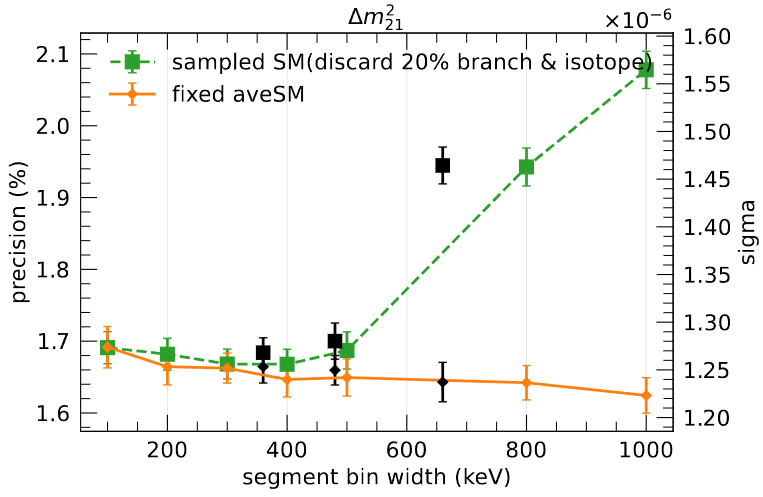
\includegraphics[width=\linewidth]{5_oscillation/segment_dmsq21.png}
    \caption{}
    \label{fig:segment_dmsq21}
  \end{subfigure}
  \hfill
  \begin{subfigure}[t]{0.45\textwidth}
    \centering
    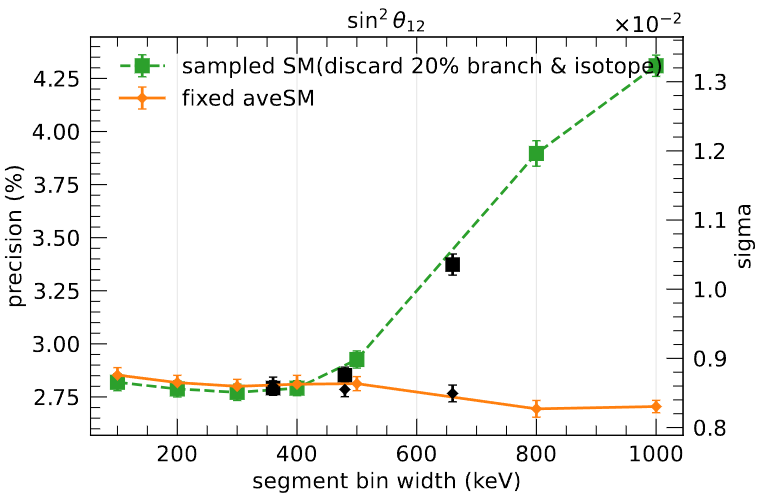
\includegraphics[width=\linewidth]{5_oscillation/segment_sinsq12.png}
    \caption{}
    \label{fig:segment_sinsq12}
  \end{subfigure}
  \caption{Precision of (a) $\Delta m^2_{21}$ and (b) $\sin^2\theta_{12}$ as a function of reactor-spectrum segment width. Green markers/lines show results when the Summation Model is perturbed (randomly discarding 20\% of branches/isotopes); orange markers/lines indicate the baseline precision with a fixed average Summation Model. Black points correspond to segmentation defined by the detector energy resolution (energy-resolution-driven segmentation), while the colored-line points correspond to uniform segmentation of the reactor spectrum. Error bars denote the statistical uncertainty from repeated toys/fits. The additional model-dependent systematic uncertainty is minimized at a segment width of approximately 300\,keV, indicating an optimal trade-off between model flexibility and available statistical constraint.
}
\end{figure}

Figures \ref{fig:segment_dmsq21} and \ref{fig:segment_sinsq12} demonstrate that the additional model-dependent systematic uncertainty is minimized at a segment width of approximately \(300\,\mathrm{keV}\): around this point the difference between the green and orange curves is smallest, indicating effective suppression of model-related uncertainty. Conversely, overly fine segmentation weakens Daya Bay (DYB)'s statistical constraint on each segment and can increase statistical noise or inter-segment correlations, potentially leading to overfitting; overly coarse segmentation cannot absorb local shape differences, causing the model-dependent systematic to grow. Under the perturbation assumptions adopted here, a segment width of about \(300\,\mathrm{keV}\) provides a favorable compromise between reducing model-dependent bias and maintaining adequate statistical constraint.



\subsubsection{Summation Model}

 Currently, the commonly used methods for calculating reactor neutrino flux include the conversion method and the summation method. In recent years, with the continuous improvement and updating of nuclear data, as well as the application of total absorption γ-ray spectroscopy technology, the measurement of β-decay branching data has become more accurate. Consequently, the reliability of neutrino flux models derived via the summation method has been significantly enhanced. The summation method can provide a direct explanation for the reactor neutrino anomaly.

The calculation process of the summation method, as illustrated in the Figure~\ref{fig:summation_procedure}, consists primarily of two components: nuclear database inputs and antineutrino spectra calculation for individual β-decay branches. Further details can be found in Xinzhao’s doctoral dissertation.
 




 \begin{figure}
     \centering
     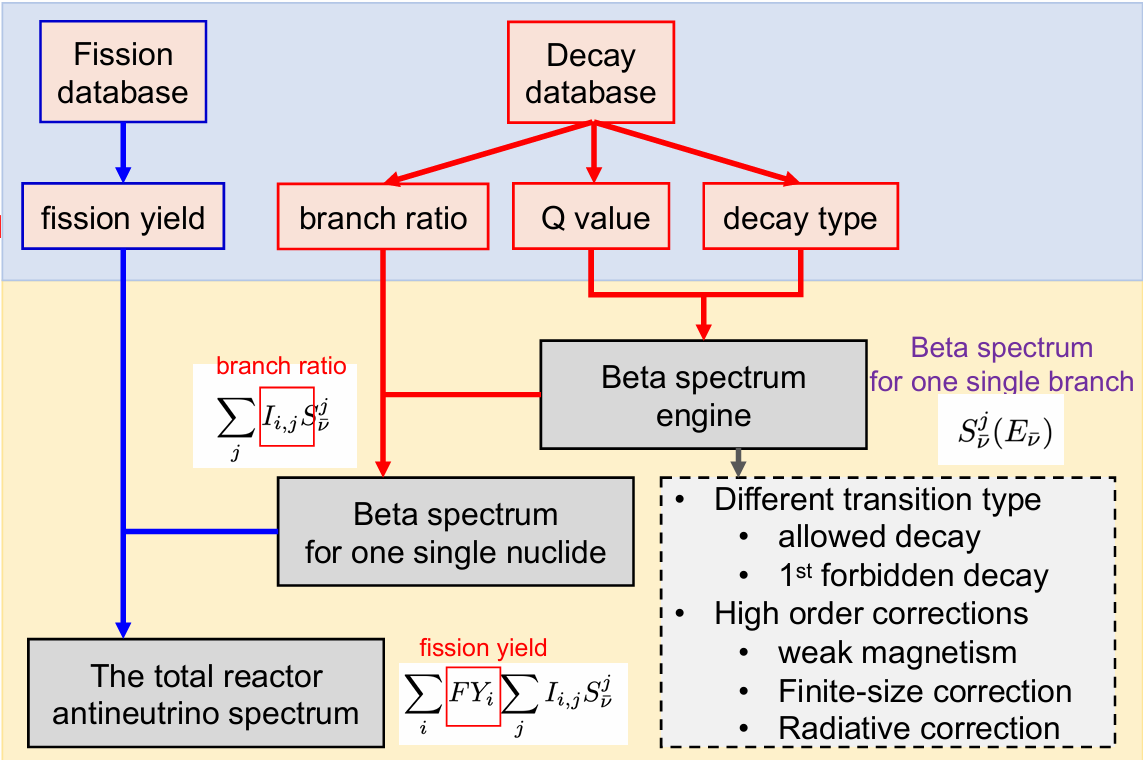
\includegraphics[width=0.75\linewidth]{5_oscillation/summation_procedure.png}
     \caption{Summation spectra calculation framework. The blue region corresponds to the nuclear database inputs, and the yellow region denotes the calculation process of the spectra calculation.}
     \label{fig:summation_procedure}
 \end{figure}

 To investigate the systematic errors in oscillation parameters induced by uncertainties in the shape of the neutrino flux spectrum, it is necessary to construct neutrino spectra with different shapes. This requirement can be achieved by randomly omitting β spectra during the construction of neutrino spectra using the summation method. The specific details are as follows:

\begin{itemize}
  \item Randomly omit $10\% (20\%) $ of the nuclides from all nuclides.
  \item Randomly omit $10\% (20\%) $ the β-decay branches from the remaining nuclides.
  \item Normalize the resulting neutrino spectrum shape to the IBD yield corresponding to the scenario where no nuclides or β-decay branches are omitted.

\end{itemize}

The average spectrum and 1 $\sigma$range of the summation model obtained via the aforementioned method are shown in the Figure~\ref{fig:sm}.
\begin{figure}[htbp] 
    \centering
   
    \begin{subfigure}[t]{0.45\textwidth}
        \centering
        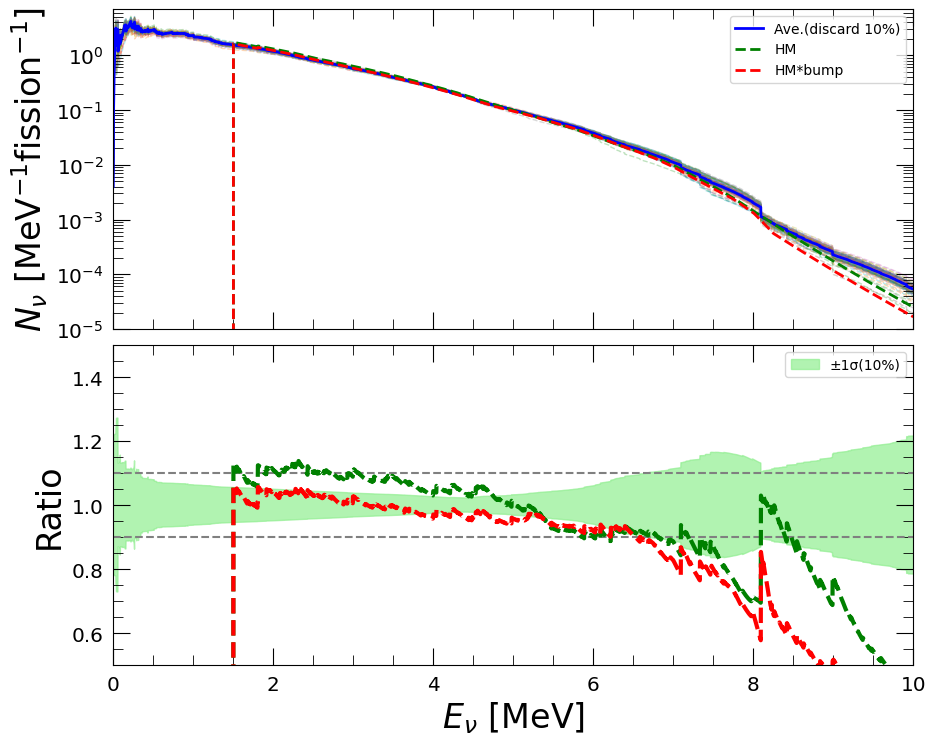
\includegraphics[width=\linewidth]{5_oscillation/sm_discard_0.1.png}
        \caption{Omit 10$\%$} 
        \label{fig:sm_0.1}
    \end{subfigure}
    \hfill  
    \begin{subfigure}[t]{0.45\textwidth}
        \centering
        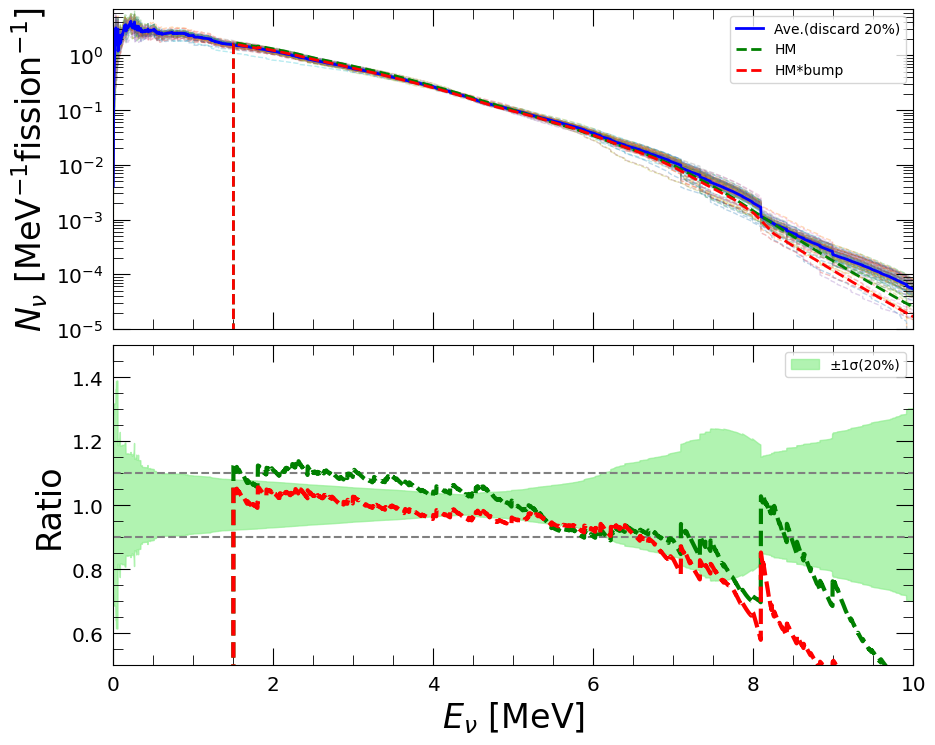
\includegraphics[width=\linewidth]{5_oscillation/sm_0.2.png}
        \caption{Omit 20$\%$}
        \label{fig:sm_0.2}
    \end{subfigure}
    \caption{average spectrum and 1$\sigma$ range of the summation model} 
    \label{fig:sm} 
\end{figure}
\subsection{Feldman-Cousins method}


To validate the use of Wilks' theorem and to obtain confidence intervals with correct coverage in non-regular situations, we performed a series of Feldman--Cousins (FC) coverage studies for the oscillation parameters of interest.  The studies include both a two-dimensional FC construction for the solar-sector parameters and a one-dimensional FC construction for $\Delta m^2_{31}$.

\subsubsection{2D Feldman--Cousins for \(\Delta m^2_{21}\) and \(\sin^2\theta_{12}\)}
We constructed an empirical distribution of the test statistic
\[
\Delta\chi^2(\delta) \equiv \chi^2(\delta) - \chi^2_{\min},
\]
by generating ensembles of pseudo-experiments (toys) under the nominal hypothesis and refitting each toy according to the standard Feldman--Cousins (FC) prescription. For the two-dimensional parameter space \((\Delta m^2_{21},\,\sin^2\theta_{12})\), the expected asymptotic behaviour of the test statistic follows a $\chi^2$ distribution with two degrees of freedom.

Figure~\ref{fig:FC21} shows the empirical $\Delta\chi^2$ distribution obtained at a representative grid point in the \((\Delta m^2_{21},\,\sin^2\theta_{12})\) plane. The extracted critical value at 68.27\% C.L.\ is consistent with the Wilks expectation within statistical uncertainties. Therefore, for the solar-sector parameters \((\Delta m^2_{21},\sin^2\theta_{12})\), the Wilks approximation is adequate in the tested region.

\begin{figure}[h]
    \centering
    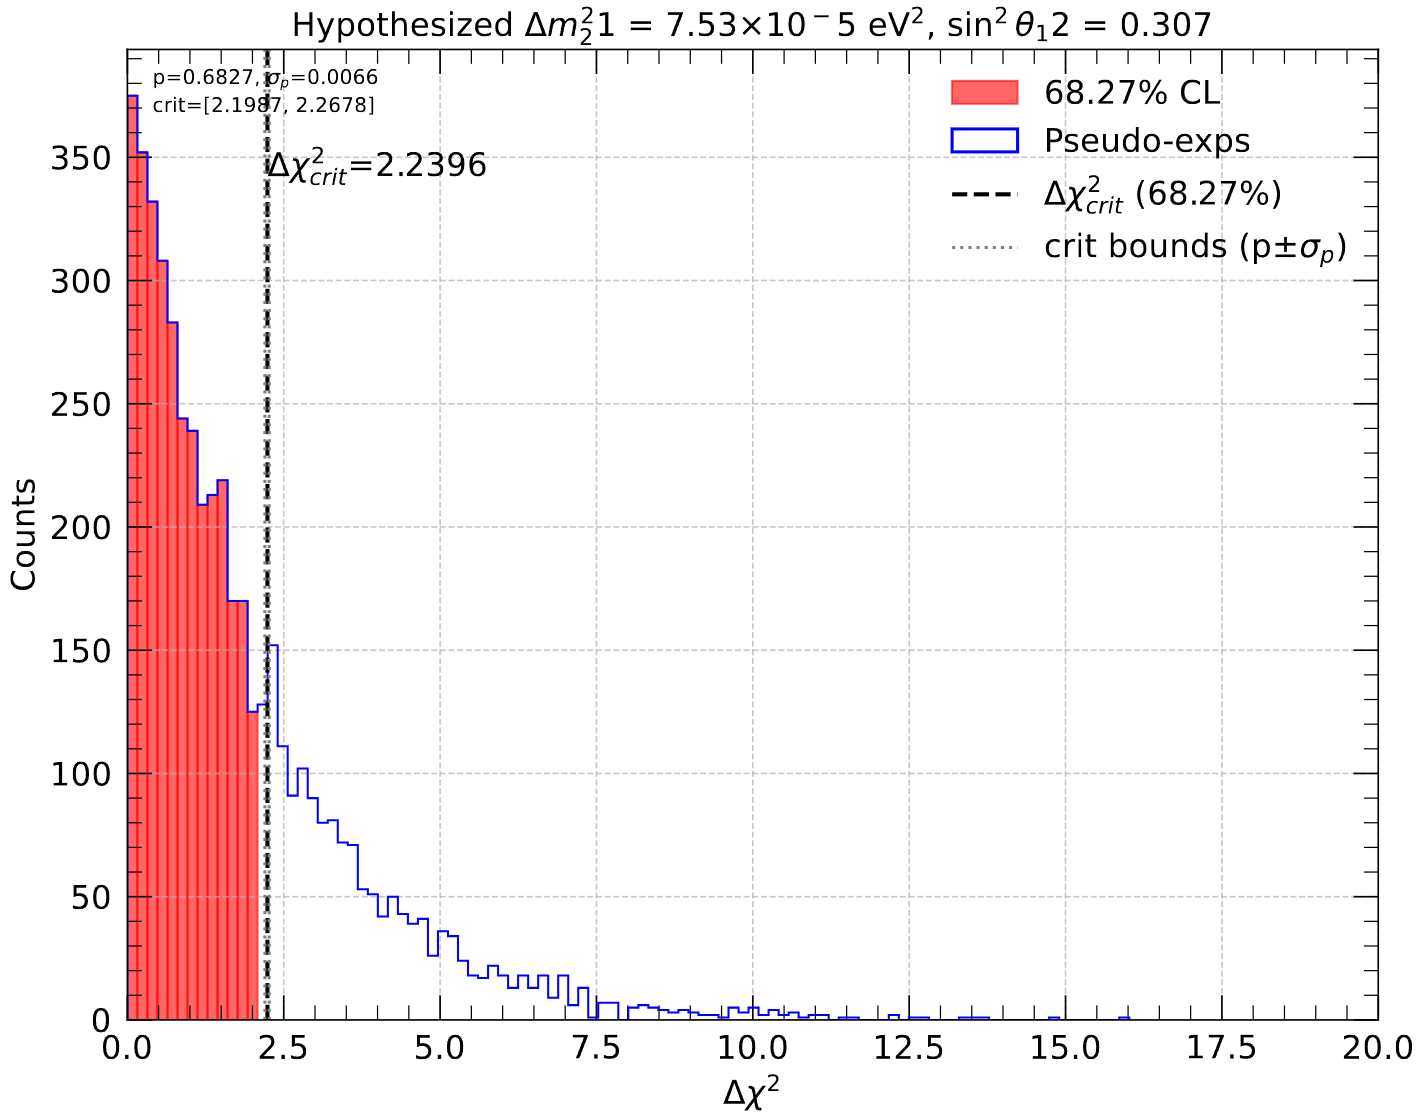
\includegraphics[width=0.7\linewidth]{5_oscillation/FC21.png}
    \caption{Empirical $\Delta\chi^2$ distribution from the 2D Feldman--Cousins test at a representative point in the \((\Delta m^2_{21},\,\sin^2\theta_{12})\) parameter space. The vertical dashed line indicates the critical value at 68.27\% C.L., which agrees with the Wilks expectation of a two-degrees-of-freedom $\chi^2$ distribution.}
    \label{fig:FC21}
\end{figure}


\subsubsection{1D Feldman--Cousins for \(\Delta m^2_{31}\)}
By contrast, the likelihood surface for \(\Delta m^2_{31}\) exhibits non-regular behaviour (nearby unphysical minima and phase-degeneracy effects) that invalidates the naive Wilks approximation in the JUNO-only configuration. We therefore applied a one-dimensional FC construction for \(\Delta m^2_{31}\). The FC procedure was carried out in two steps to assess the impact of reactor-spectrum model uncertainty:

\begin{enumerate}
  \item \textbf{Fixed reactor model:} With the reactor spectrum fixed to the average Summation Model (no shape perturbation), we generated toy ensembles and computed the empirical distribution of $\Delta\chi^2$. The resulting critical value for the 68.27\% acceptance region is
  \[
    \Delta\chi^2_{\rm crit,\,fixed} = 1.5379,
  \]
  which yields a \(\Delta m^2_{31}\) precision of \(1.39\%\) (for the 50-day exposure). The distribution of per-toy precision for this fixed-model case is shown in Fig.~\ref{fig:dmsq31_fixedaveSM}.
  \item \textbf{Sampled reactor model:} To include reactor-model variation we sampled an ensemble of perturbed reactor spectra by varying each 20-keV segment (the sampled-model ensemble, $N_{\rm toys}=5000$), and repeated the FC construction using these perturbed models. The empirical critical value becomes
  \[
    \Delta\chi^2_{\rm crit,\,sampled} = 1.5724,
  \]
  corresponding to a \(\Delta m^2_{31}\) precision of \(1.40\%\) (50-day exposure). The per-toy precision distribution for the sampled (Gaussian-perturbed) models is shown in Fig.~\ref{fig:dmsq31_gaussian}.
\end{enumerate}

The critical value increases slightly when using the sampled reactor-model ensemble compared to the fixed model. The observed difference is small; moreover, the uncertainty on the empirical critical values can be reduced further by increasing the number of toys in the FC ensembles.

From the above studies we draw the following conclusions:
\begin{itemize}
  \item The model-dependent systematic uncertainty affecting \(\Delta m^2_{31}\) is small: we estimate the additional systematic contribution from reactor-model variation to be \(<0.3\%\) on the \(\Delta m^2_{31}\) precision in the 50-day scenario.
  \item For all three parameters considered (\(\Delta m^2_{21}\), \(\sin^2\theta_{12}\), and \(\Delta m^2_{31}\)), the systematic uncertainty induced by realistic reactor-model variations is smaller than the statistical uncertainty for the 50-day exposure; i.e., the remaining model-dependent systematics are negligible at this exposure.
  \item The FC-derived precision for \(\Delta m^2_{31}\) under the adopted assumptions is \(\approx 1.4\%\) (50-days exposure). This is slightly worse than the global-fit precision (approximately \(1.1\%\)) but is internally consistent given the JUNO-only configuration and the treated reactor-model uncertainties.
\end{itemize}

\paragraph{Practical notes.} The FC ensembles reported above used $N_{\rm toys}=5000$ pseudo-experiments for the sampled-model case; increasing $N_{\rm toys}$ will reduce the statistical uncertainty on the empirical critical $\Delta\chi^2$ values. The FC procedure and the quoted numbers should therefore be interpreted with their toy-statistics uncertainty in mind.

\begin{figure}[!htbp]
  \centering
  \begin{subfigure}[t]{0.45\textwidth}
    \centering
    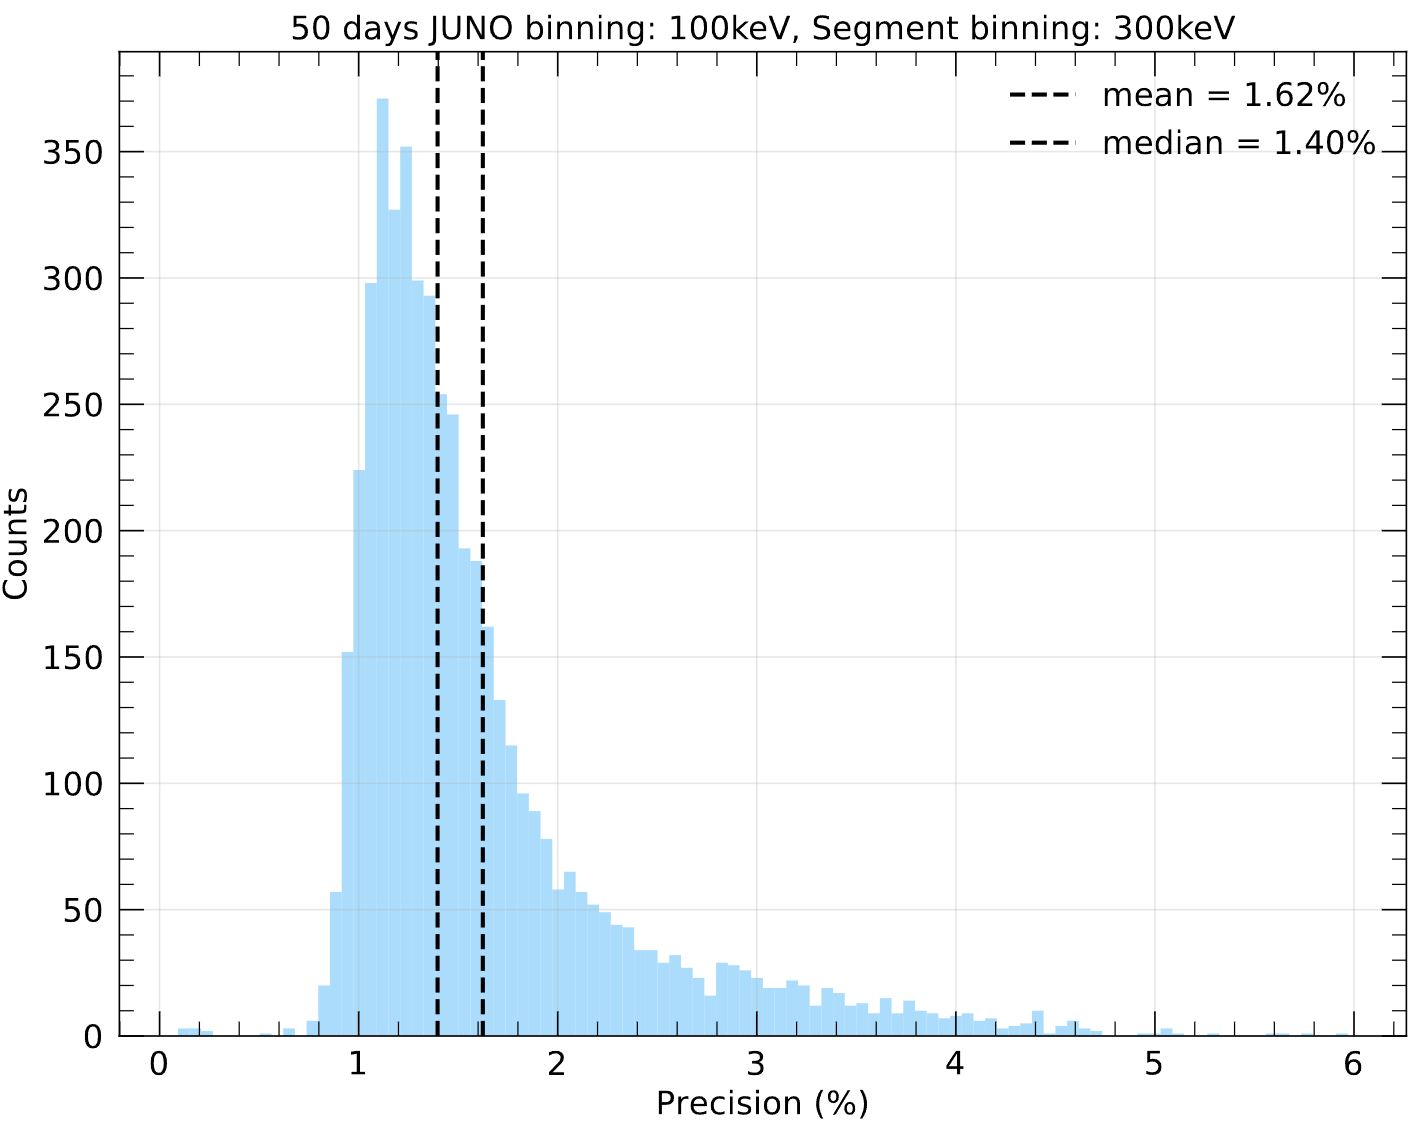
\includegraphics[width=\linewidth]{5_oscillation/dmsq31_gaussian.png}
    \caption{Per-toy precision distribution for the sampled (Gaussian-perturbed) reactor-model ensemble ($N_{\rm toys}=5000$).}
    \label{fig:dmsq31_gaussian}
  \end{subfigure}%
  \hfill
  \begin{subfigure}[t]{0.45\textwidth}
    \centering
    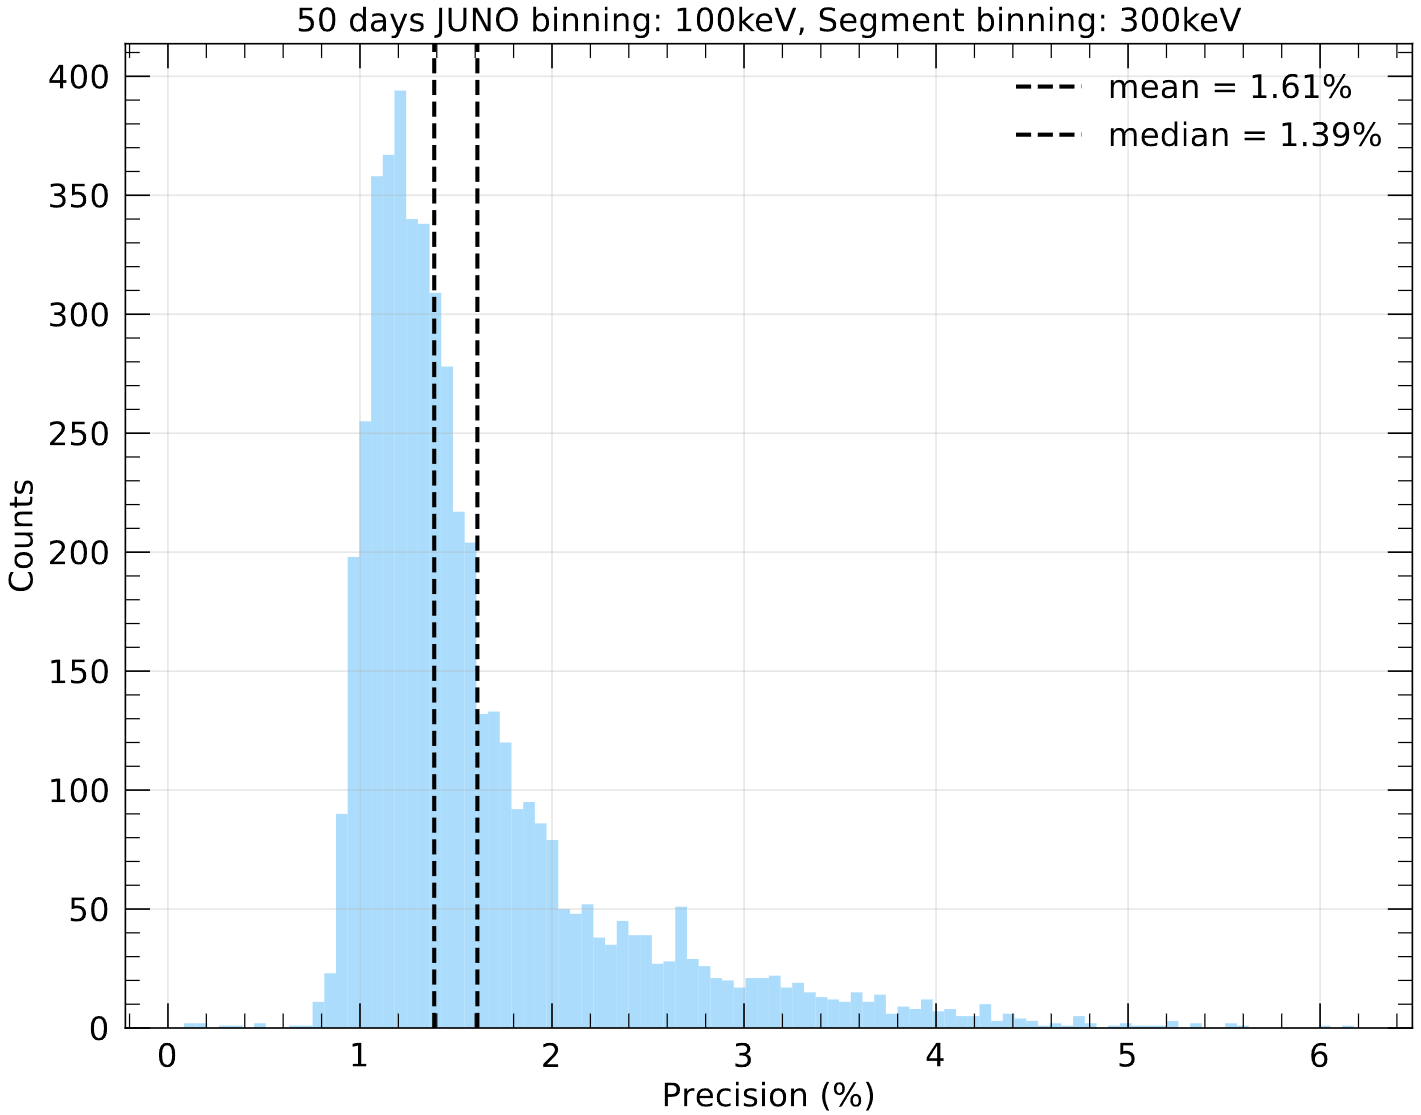
\includegraphics[width=\linewidth]{5_oscillation/dmsq31_fixedaveSM.png}
    \caption{Per-toy precision distribution for the fixed average Summation Model ($N_{\rm toys}=5000$) (no shape perturbation).}
    \label{fig:dmsq31_fixedaveSM}
  \end{subfigure}
  \label{fig:dmsq31_FC}
\end{figure}

\subsection{Oscillation analysis result}
\label{subsec:analysis:result}
Incorporating the estimates of selection efficiency, background contributions, and reactor information, the observed prompt energy spectrum of IBD candidates shown in Fig.~\ref{fig:P25C:spectrum} is compared with a detailed prediction to extract the neutrino oscillation parameters. The spectral distortion observed in the prompt-energy spectrum in Fig.~\ref{fig:P25C:spectrum} was primarily shaped by solar oscillation parameters $\Delta m_{21}^2$ and $\sin^2\theta_{12}$. 
Given the limited statistics of the current data, $\rm{sin}^2\theta_{13}=0$ cannot be strongly rejected in JUNO. However, the third oscillation pattern has already been firmly established by the Daya Bay measurements with high significance. Therefore, external constraints on $\rm{sin}^2\theta_{13}$ and $\Delta m^2_{31}$ from Daya Bay are applied by default. We find that applying or removing the $\Delta m^2_{31}$ constraint has a negligible impact on the measurement of the solar oscillation parameters $\sin^2\theta_{12}$ and $\Delta m^2_{21}$, the measurement is insensitive to the neutrino mass ordering. Due to the currently limited statistics, our oscillation analysis concentrated on determining the solar parameters. The residuals between data and the full prediction are small and consistent within 2$\sigma$, yielding a goodness of fit of $\chi^2/\rm{ndf}=63.03/64$.

\begin{figure}[!htbp]
    \centering
    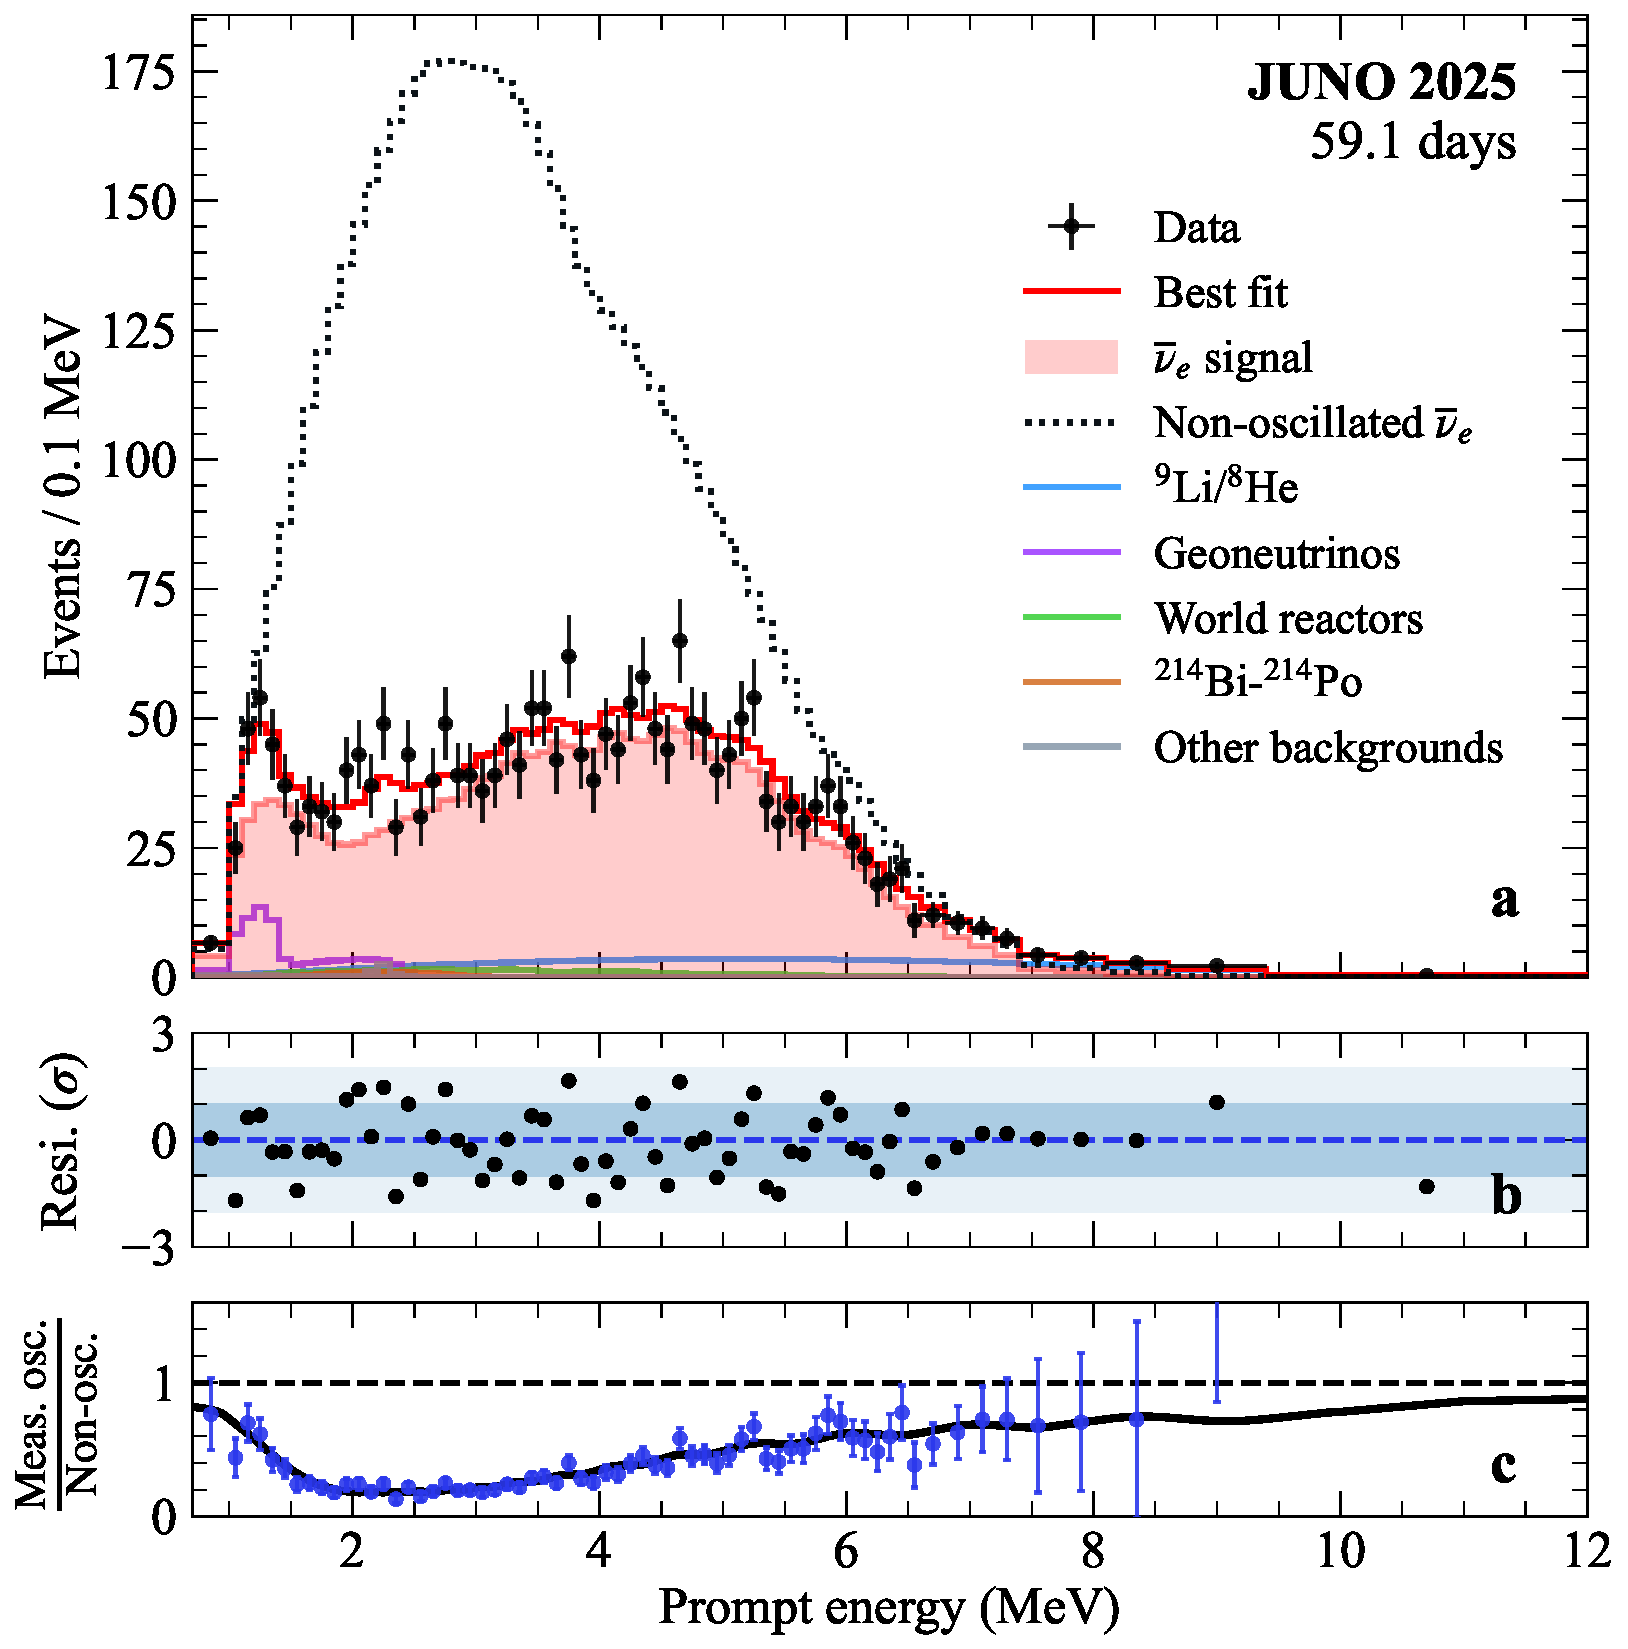
\includegraphics[width=0.65\linewidth]{5_oscillation/spectrum_component_v3.2.pdf}
    \caption{Measured energy spectrum of prompt IBD candidates. a, Black points show measured data with statistical error bars, with the red curve indicating the best-fit oscillation model. Shaded red region represents expected antineutrino signal. Black dotted line represents non-oscillated reactor neutrino expectation. Backgrounds are indicated by other solid color lines. b, Residuals quantifying the statistical consistency between data and the complete model. c, Ratio of the measured oscillated spectrum to non-oscillated prediction.}
    \label{fig:P25C:spectrum}
\end{figure}

The oscillation analysis yielded the following results for the solar parameters for normal mass ordering scenario:
\begin{equation}
\sin^2\theta_{12} &= 0.3092 \pm 0.0087 ,~~~
\Delta m_{21}^2 &= (7.50 \pm 0.12) \times 10^{-5}~\mathrm{eV}^2 .
\end{equation}
The fraction of neutron capture on carbon (99.22\%) is not included in this analysis, but it has a negligible impact on both the best-fit oscillation parameters and their precision.
The allowed regions of oscillation parameters are shown in Fig.~\ref{fig:P25C:osci}. Results from other measurements of reactor neutrinos (KamLAND~\cite{gando2013reactor} and SNO+~\cite{abreu2025measurement}) and solar neutrinos (combined Super-Kamiokande (SK)+SNO~\cite{abe2024solar}) are also shown for comparison in Fig.~\ref{fig:P25C:osci} and Fig.~\ref{fig:P25C:GlobalComp}. This result improved the precision of both parameters by a factor of 1.6.

\begin{figure}[htbp]
    \centering
    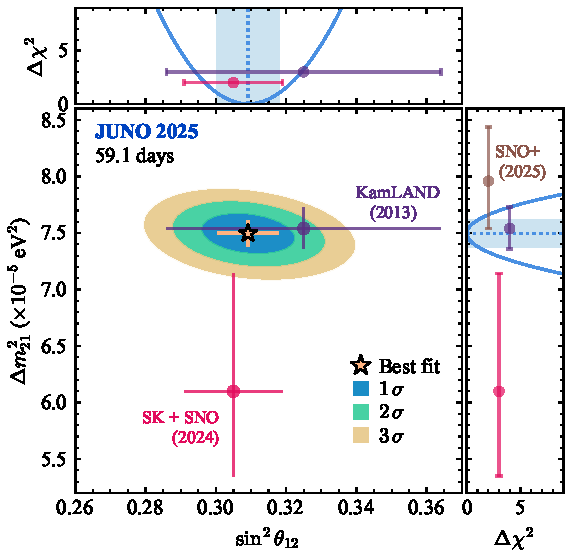
\includegraphics[width=0.65\linewidth]{5_oscillation/plot_contour_sinsq12_dmsq21_with_profiles_NO_errorbar_otherexp_v3.pdf}
    \caption{Results on solar oscillation parameters. Confidence intervals of $\sin^2\theta_{12}$ and $\Delta m_{21}^2$ obtained from the spectral fit of the prompt antineutrino energy spectrum in Fig.~\ref{fig:P25C:spectrum}. Shaded elliptical regions denote the $1\sigma$, $2\sigma$, and $3\sigma$ confidence levels ($\Delta\chi^2 = 2.30,\ 6.18,\ 11.83$). The upper panel shows the one-dimensional $\Delta\chi^2$ for $\sin^2\theta_{12}$ with $\Delta m_{21}^2$ profiled; the right panel shows the corresponding result for $\Delta m_{21}^2$ with $\sin^2\theta_{12}$ profiled. The star indicates the JUNO best-fit point, and the error bars represent the one-dimensional $1\sigma$ intervals.}
    \label{fig:P25C:osci}
\end{figure}

\begin{figure}[!htbp]
  \centering
  \begin{subfigure}[t]{0.45\textwidth}
    \centering
    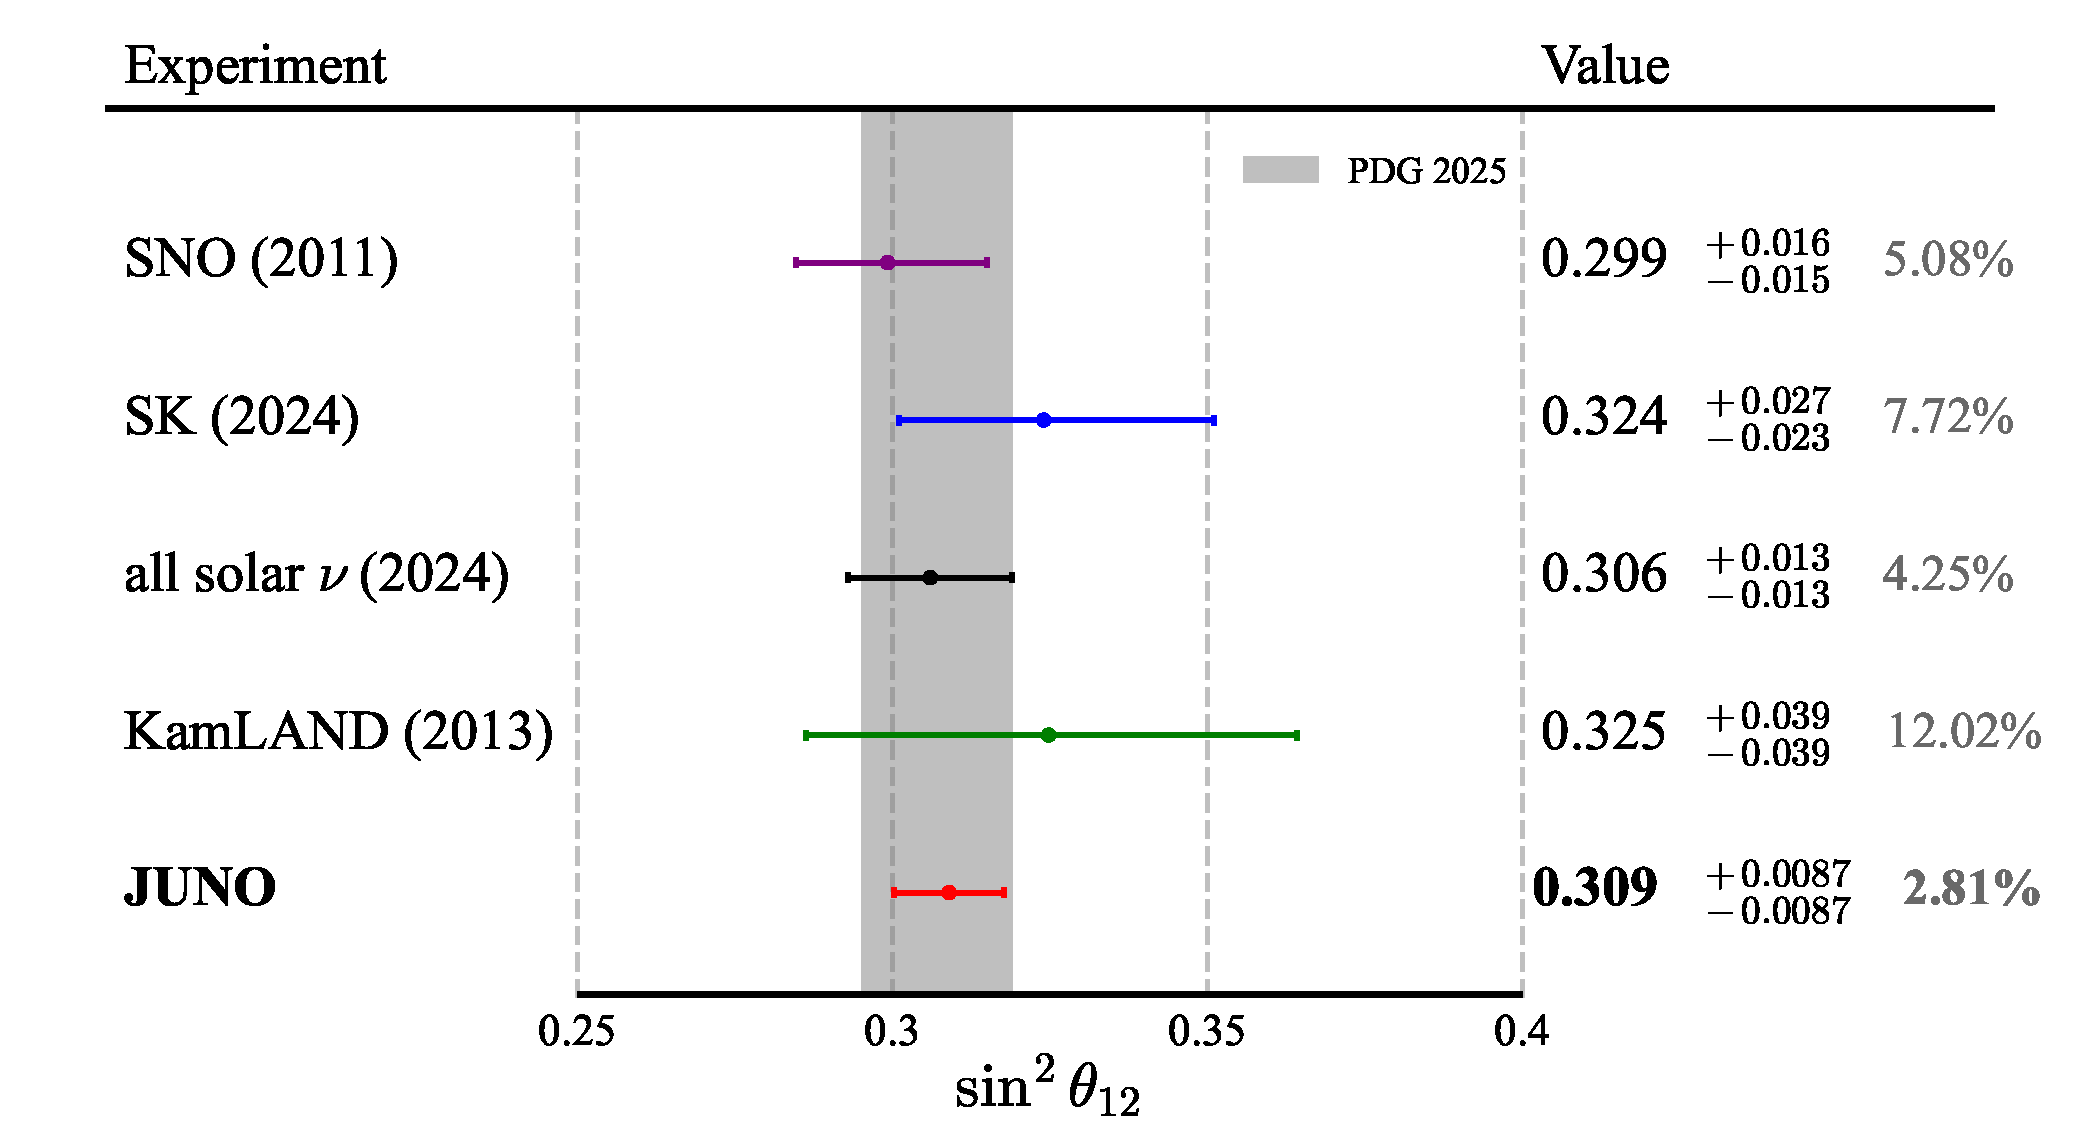
\includegraphics[width=\linewidth]{5_oscillation/th12_new_v251119_w_all_solar.pdf}
    \caption{}
    \label{fig:GlobalComp_sinsq12}
  \end{subfigure}%
  \hspace{0.02\textwidth}
  \begin{subfigure}[t]{0.45\textwidth}
    \centering
    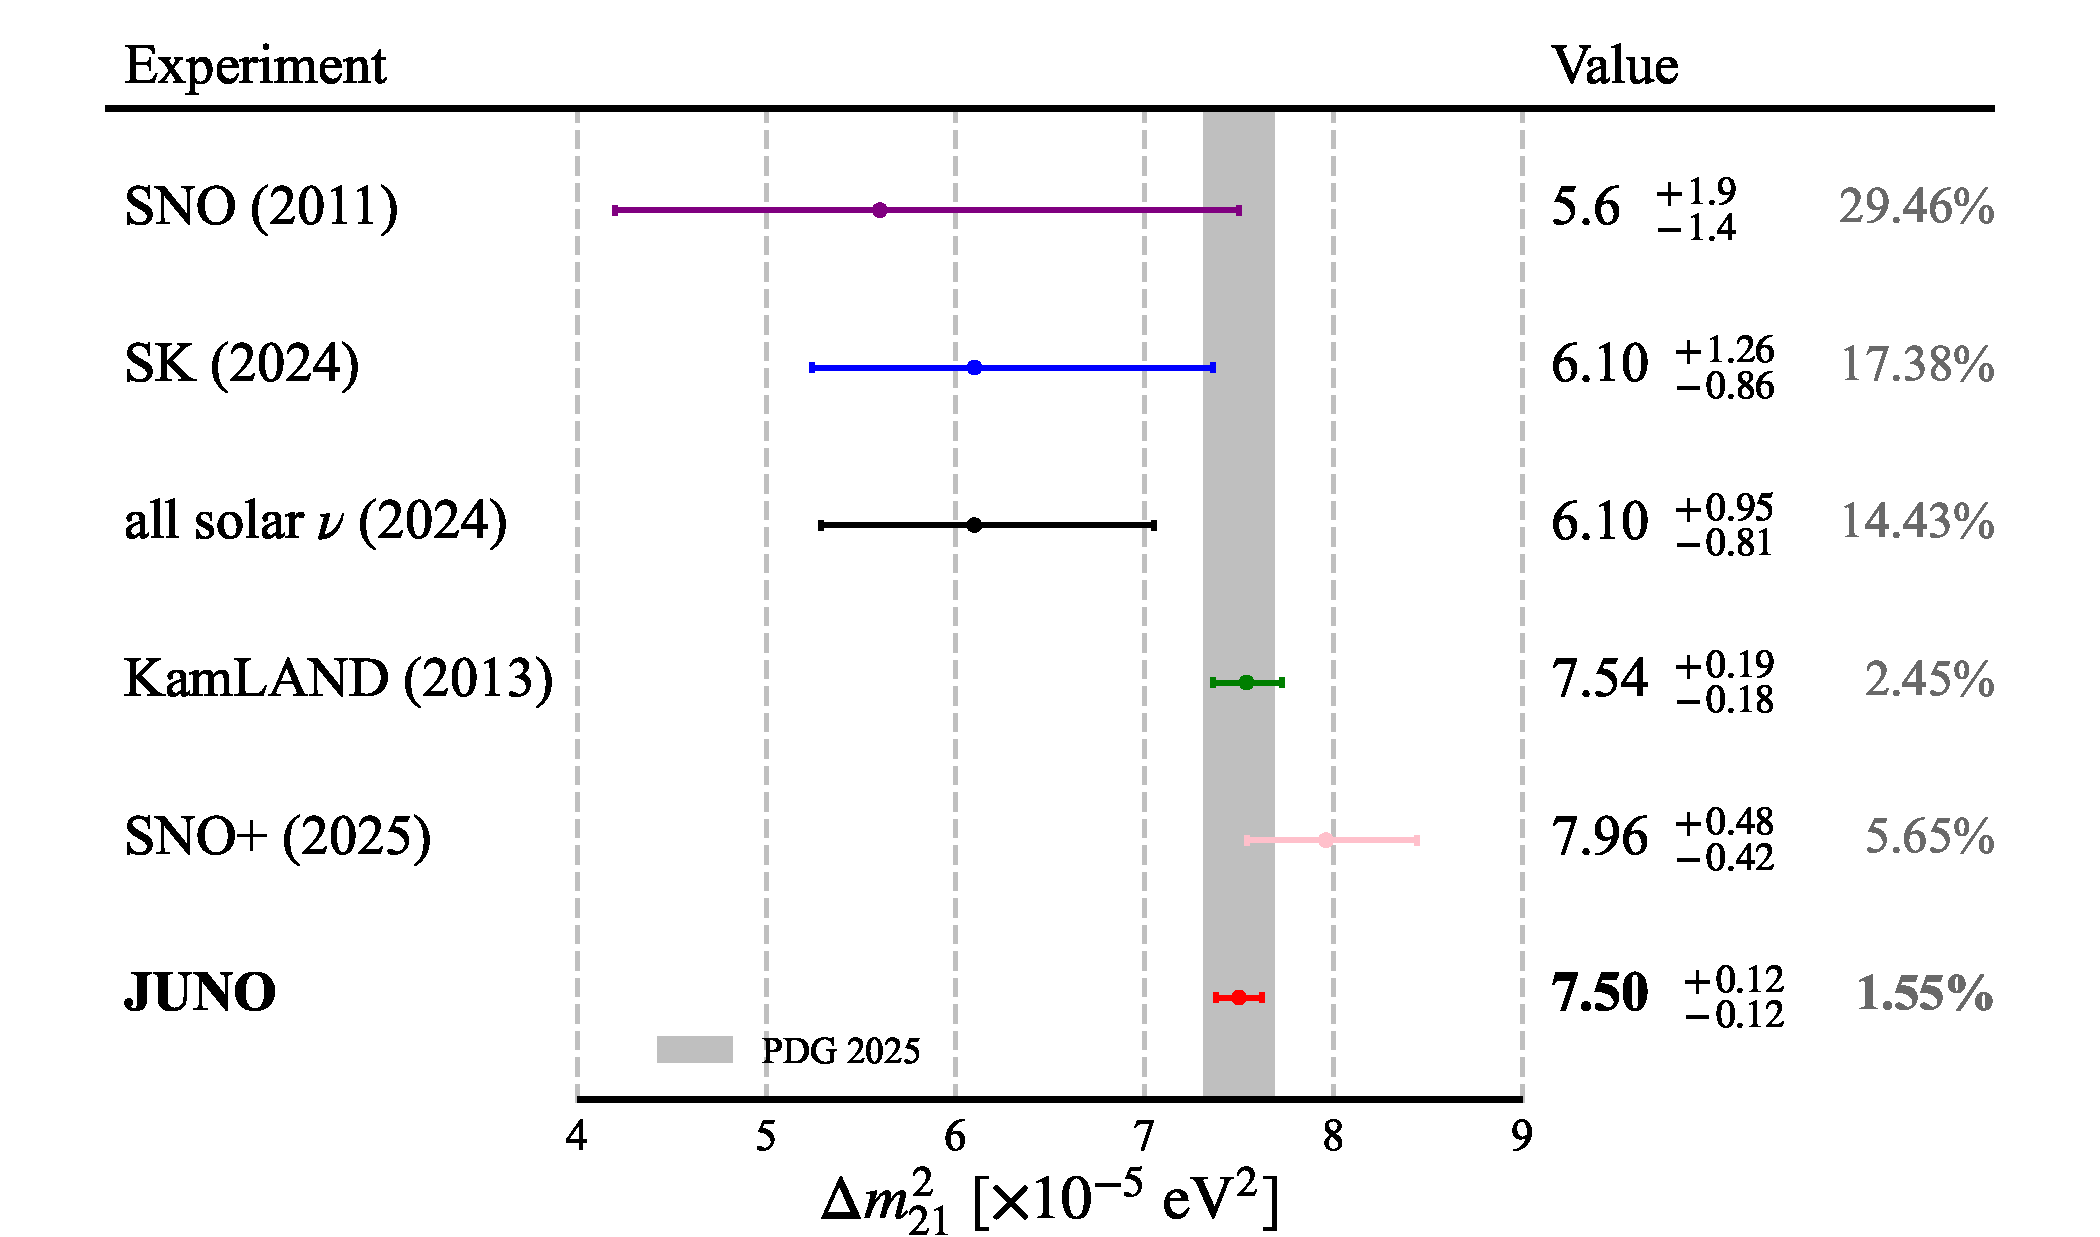
\includegraphics[width=\linewidth]{5_oscillation/m21_v251119_sno+_prl_w_all_solar.pdf}
    \caption{}
    \label{fig:GlobalComp_dmsq21}
  \end{subfigure}
  \caption{Global comparisons of $\sin^2\theta_{12}$ and $\Delta m_{21}^2$ between JUNO and other experiments, together with the PDG 2025 values, are shown in Fig.~\ref{fig:GlobalComp_sinsq12} and Fig.~\ref{fig:GlobalComp_dmsq21}, respectively.}
  \label{fig:P25C:GlobalComp}
\end{figure}

The resulting time evolution of the predicted IBD rate, compared to the measured rate with backgrounds subtracted, is shown in Fig.~\ref{fig:P25C:rate_time_evolution}; the observed variations closely track the known reactor power history. 
% To clearly illustrate the oscillation pattern, we compute the preliminary $L_{\rm eff}/E_\nu$ spectrum shown in Fig.~\ref{fig:P25C:LOverE}, where $L_{\rm eff}$ denotes the flux-weighted baseline of the YJ and TS reactor cores, and the neutrino energy is approximated as $E_\nu \approx E_{\rm rec}+0.784~\rm{MeV}$. The data points are consistent with the predicted oscillation probability, except for the point at large $L/E$, which corresponds to a reconstructed energy of around 3 MeV. The origin of this deviation is under investigation.
\begin{figure}[htbp]
    \centering
    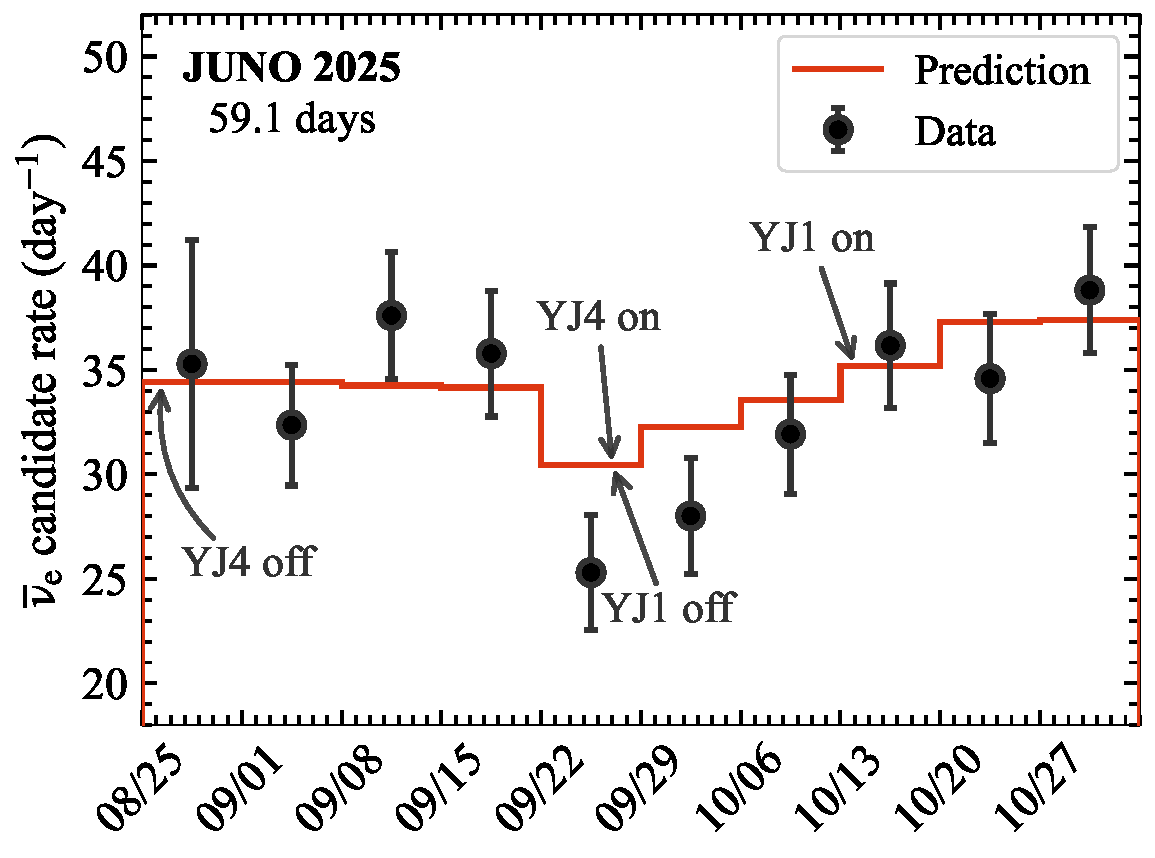
\includegraphics[width=0.65\linewidth]{5_oscillation/IBD_rate_time_evolution.pdf}
    \caption{Temporal distribution of reactor neutrinos. Rates of antineutrino candidates (after subtraction of the mean background rates), shown in one-week time bins (black points with statistical error) are compared to the prediction (red line). Arrows indicate operations on the cores YJ1 and YJ4 of the Yangjiang NPP. The NPP reduced the power output due to the occurrence}
    \label{fig:P25C:rate_time_evolution}
\end{figure}

% \begin{figure}[!htbp]
%     \centering
%     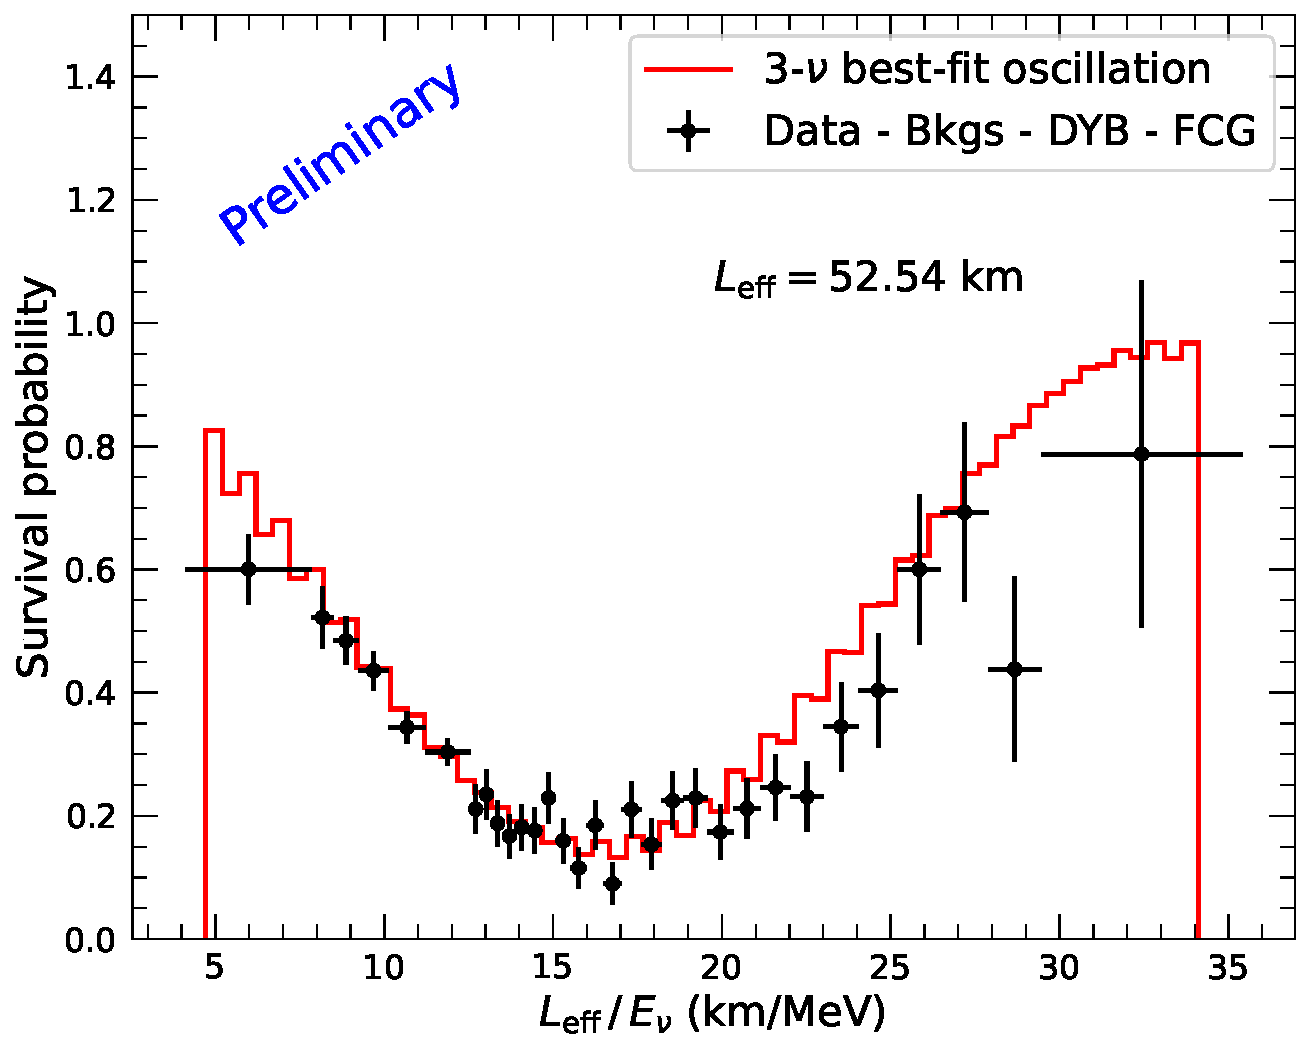
\includegraphics[width=0.65\linewidth]{5_oscillation/Leff_over_Enu_spec.pdf}
%     \caption{Measured $L/E$ spectrum of prompt IBD candidates from the YJ and TS reactor cores. Backgrounds and the IBD contributions from DYB and FCG have been subtracted. The red curve shows the expected three-neutrino survival probability calculated with the best-fit oscillation parameters.}
%     \label{fig:P25C:LOverE}
% \end{figure}

% \subsection{Error budget}

% \begin{figure}[h]
%   \centering
%   \begin{subfigure}[t]{0.32\textwidth}
%     \centering
%     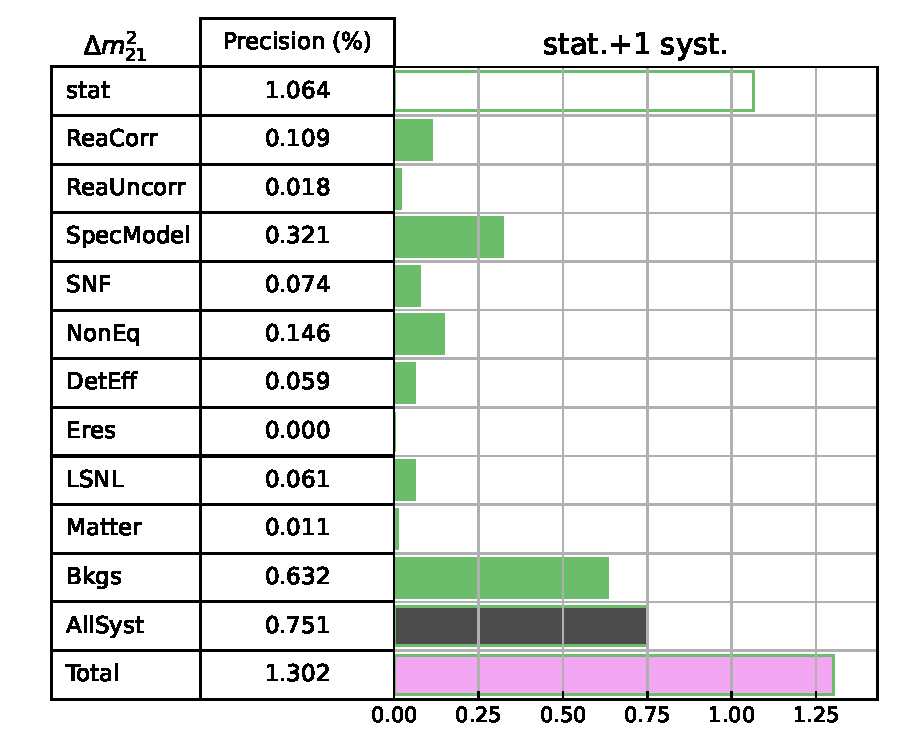
\includegraphics[width=\linewidth]{5_oscillation/dmsq21_50ds_juno_only.pdf}
%     \caption{50 days}
%     \label{fig:l1}
%   \end{subfigure}
%   \hfill
%   \begin{subfigure}[t]{0.32\textwidth}
%     \centering
%     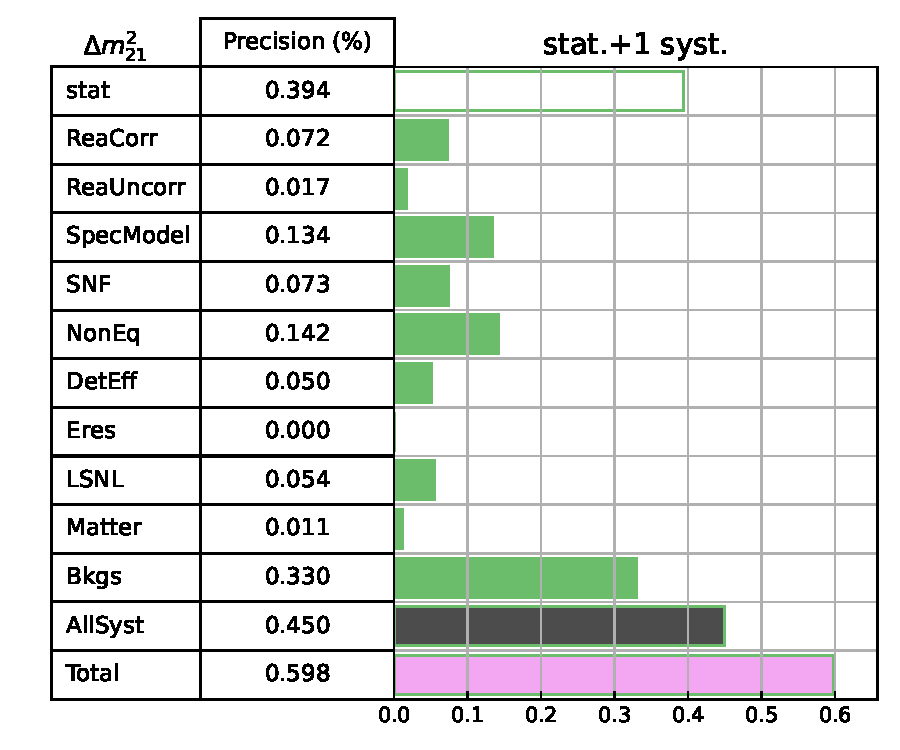
\includegraphics[width=\linewidth]{5_oscillation/dmsq21_1yr_juno_only.pdf}
%     \caption{1 year}
%     \label{fig:l2}
%   \end{subfigure}
%   \hfill
%   \begin{subfigure}[t]{0.32\textwidth}
%     \centering
%     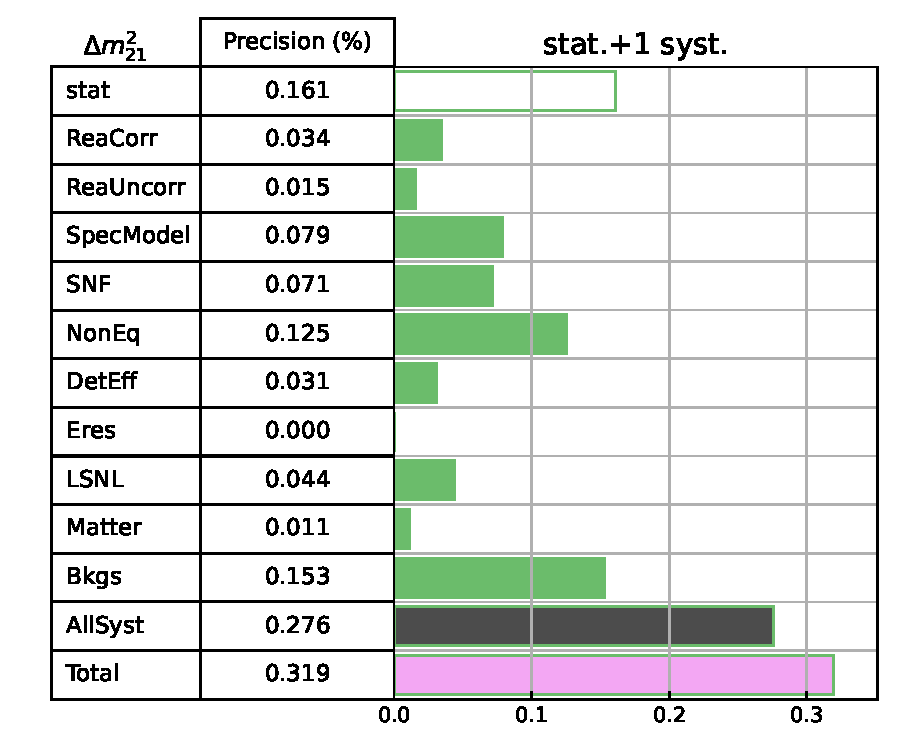
\includegraphics[width=\linewidth]{5_oscillation/dmsq21_6yr_juno_only.pdf}
%     \caption{6 years}
%     \label{fig:l3}
%   \end{subfigure}
%   \caption{Precision breakdown of $\rm \Delta m^2_{21}$}
%   %\label{Precision breakdown of $\rm \Delta m^2_{21}$}
% \end{figure}

% \begin{figure}[h]
%   \centering
%   \begin{subfigure}[t]{0.32\textwidth}
%     \centering
%     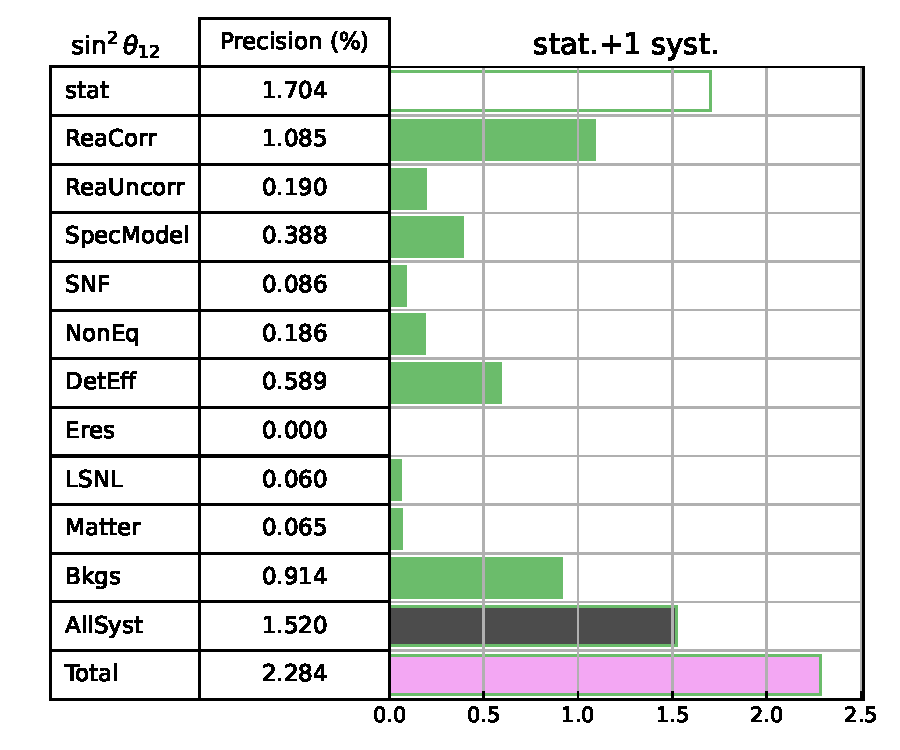
\includegraphics[width=\linewidth]{5_oscillation/sinsq12_50ds_juno_only.pdf}
%     \caption{50 days}
%     \label{fig:l1}
%   \end{subfigure}
%   \hfill
%   \begin{subfigure}[t]{0.32\textwidth}
%     \centering
%     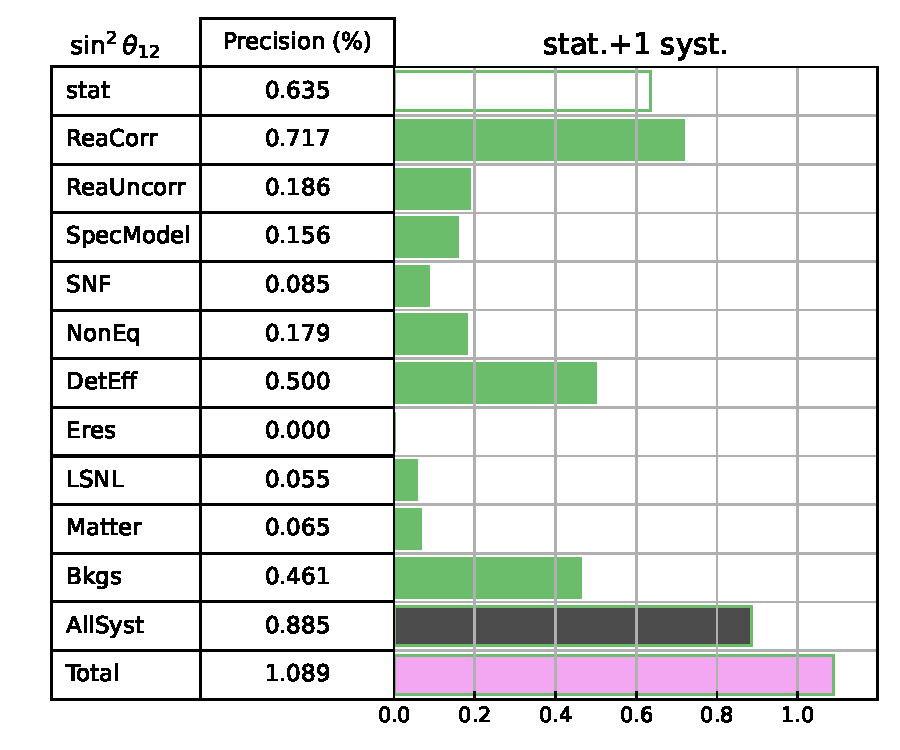
\includegraphics[width=\linewidth]{5_oscillation/sinsq12_1yr_juno_only.pdf}
%     \caption{1 year}
%     \label{fig:l2}
%   \end{subfigure}
%   \hfill
%   \begin{subfigure}[t]{0.32\textwidth}
%     \centering
%     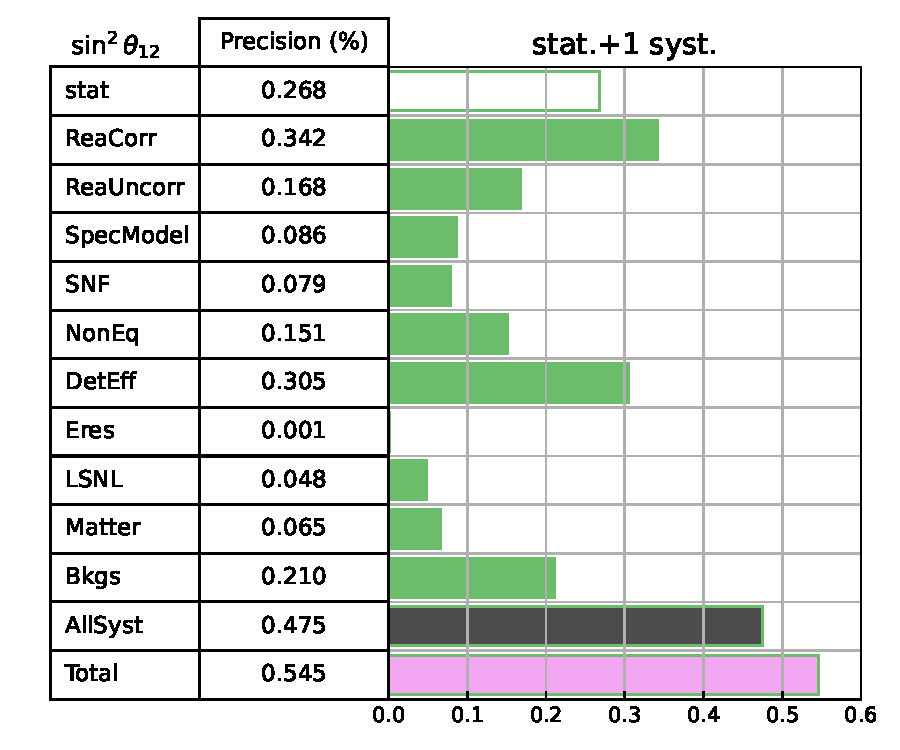
\includegraphics[width=\linewidth]{5_oscillation/sinsq12_6yr_juno_only.pdf}
%     \caption{6 years}
%     \label{fig:l3}
%   \end{subfigure}
%   \caption{Precision breakdown of $\rm sin^2\theta_{12}$.}
%   %\label{Precision breakdown of $\rm sin^2\theta_{12}$}
% \end{figure}

% \begin{figure}[h]
%   \centering
%   \begin{subfigure}[t]{0.32\textwidth}
%     \centering
%     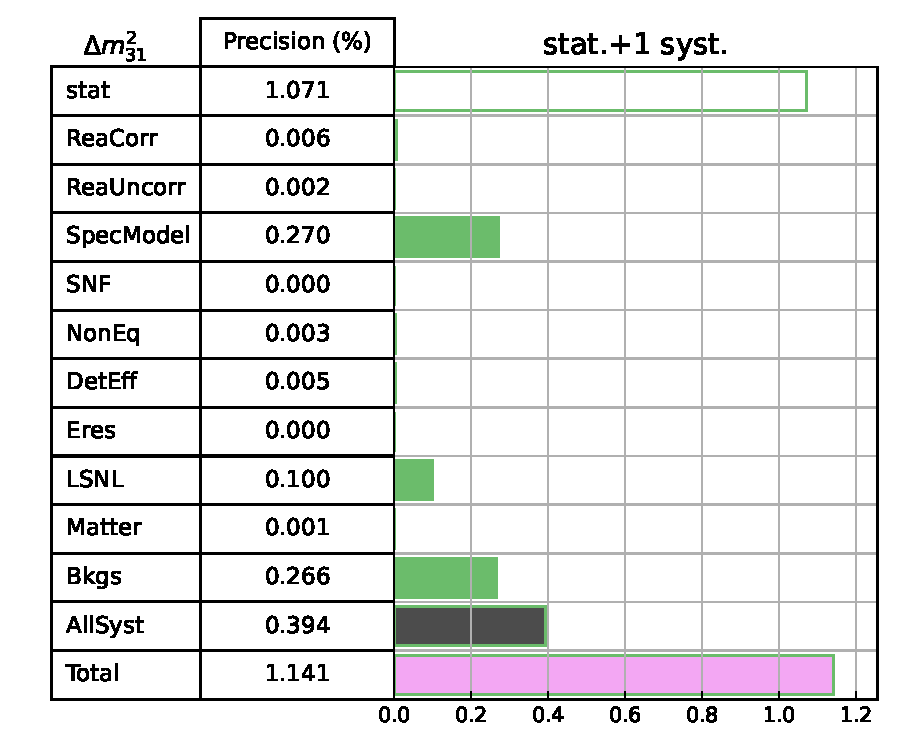
\includegraphics[width=\linewidth]{5_oscillation/dmsq31_50ds_juno_only.pdf}
%     \caption{50 days}
%     \label{fig:l1}
%   \end{subfigure}
%   \hfill
%   \begin{subfigure}[t]{0.32\textwidth}
%     \centering
%     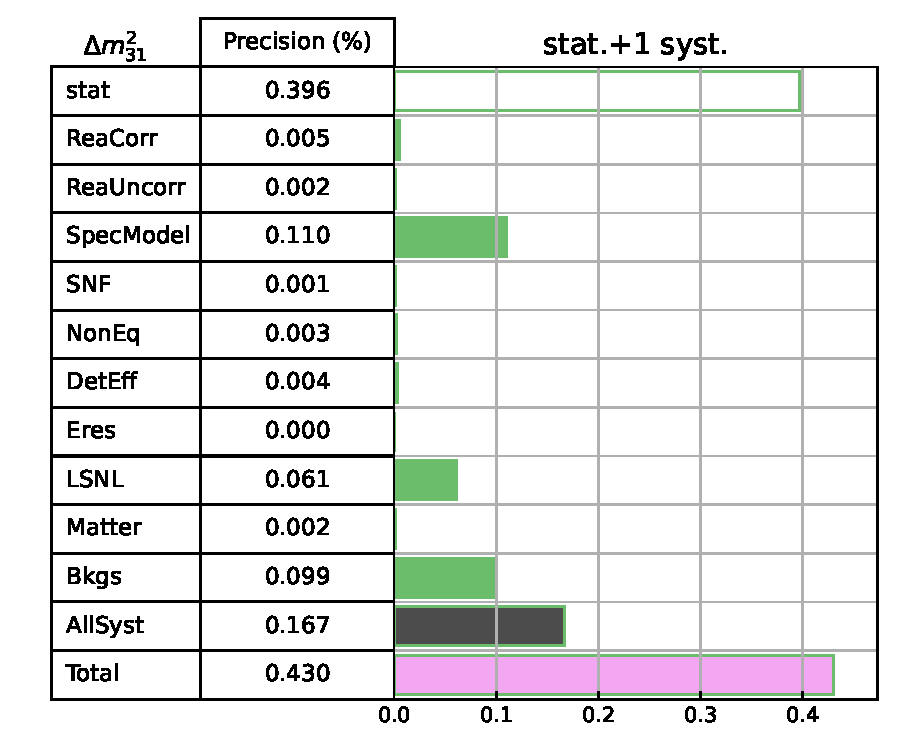
\includegraphics[width=\linewidth]{5_oscillation/dmsq31_1yr_juno_only.pdf}
%     \caption{1 year}
%     \label{fig:l2}
%   \end{subfigure}
%   \hfill
%   \begin{subfigure}[t]{0.32\textwidth}
%     \centering
%     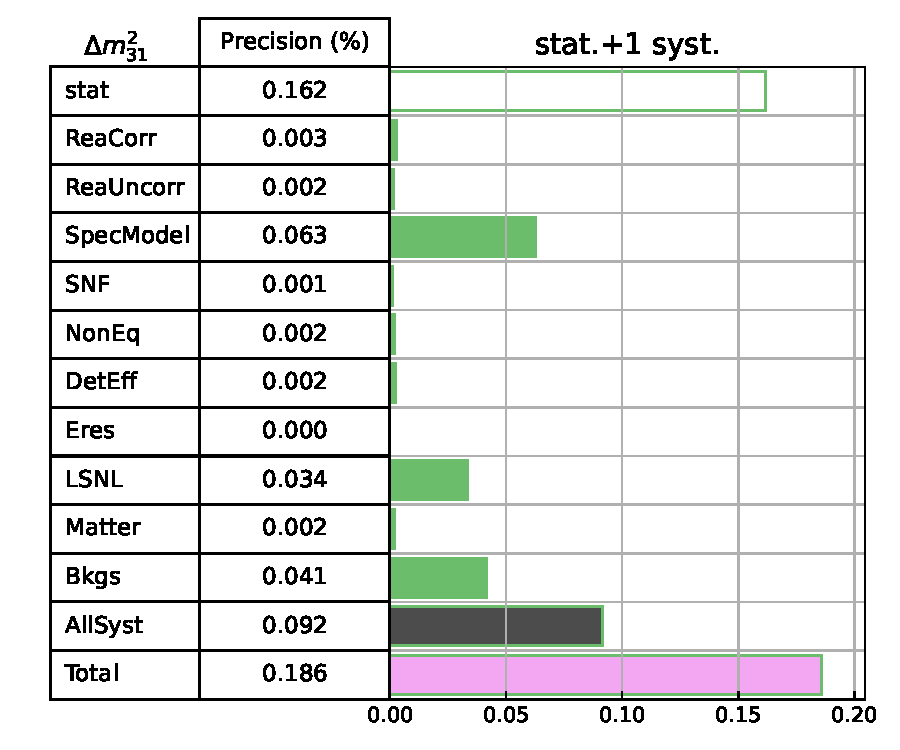
\includegraphics[width=\linewidth]{5_oscillation/dmsq31_6yr_juno_only.pdf}
%     \caption{6 years}
%     \label{fig:l3}
%   \end{subfigure}
%   \caption{Precision breakdown of $\rm \Delta m^2_{31}$}
%   %\label{Precision breakdown of $\rm \Delta m^2_{31}$}
% \end{figure}